
%%%% Uncomment the first group of lines for llncs formatting
%%%% Uncomment the second group of lines for non-llncs formatting

% not sim(s1,s2,e1) iff
% either there is a delta <= C
%     exec(s1,e1,delta) and not ||{e2} exec(s2, e2,delta)j=
% or there is a delta > C
%
%

% \documentclass[10pt, twocolumn]{article}
\documentclass[11pt]{article}
% \documentclass[10pt, conference, compsocconf]{IEEEtran}
% \newcommand{\usellncs}[2]{{#1}}
% \documentclass[11pt]{llncs}


\usepackage[T1]{fontenc}
\usepackage{algorithmic}
\usepackage{algorithm}
\usepackage{complexity}
\usepackage{times}
\usepackage{graphicx}
\usepackage{multirow}
\usepackage{slashbox}
\usepackage{tabularx}

% \newdef{definition}{Definition}
\newtheorem{theorem}{Theorem}
\newtheorem{lemma}[theorem]{Lemma}
\newtheorem{corollary}[theorem]{Corollary}
% \newtheorem{lemma}{Lemma}
\newtheorem{proposition}[theorem]{Proposition}
% \newtheorem{example}[theorem]{Example}
\newtheorem{definition}{Definition}
% \newdef{definition}{Definition}
\newtheorem{example}{Example}
% \newenvironment{proof}{\noindent\par{\bf Proof: }}{\nopagebreak\rule{1 ex}{0.8 em}\medskip}
\addtolength{\textheight}{1.0in}
\addtolength{\textwidth}{2.0in}
\addtolength{\topmargin}{-0.5in}
\addtolength{\evensidemargin}{-1in}
\addtolength{\oddsidemargin}{-1in}
% \setlength\parindent{0in}
% \setlength\parskip{0in}



\usepackage{cite}
\usepackage{amsmath}
\usepackage{amssymb}
%\usepackage{psfig}
\usepackage{epsfig}
\usepackage{color}

%%%%%%%%%%%%%%%%%%%%%%%%%%%%%%%%%%%%%%%%%%%%%%%%%%%%%%%%%%%%%%%%%
%% The following definitions are to extend the LaTex algorithmic 
%% package with SWITCH statements and one-line structures.  
%% The extension is by 
%%   Prof. Farn Wang 
%%   Dept. of Electrical Engineering, 
%%   National Taiwan University. 
%% 
\newcommand{\IFNLINE}[1]{\STATE {\bf if} #1 {\bf then} }
\newcommand{\IFLINE}[1]{{\bf if} #1 {\bf then} }
\newcommand{\ELSELINE}{\textbf{else} }
\newcommand{\ELSNLINE}{\STATE \textbf{else} }
\newcommand{\ENDIFLINE}{\textbf{end if}}
\newcommand{\ENDIFNLINE}{\STATE \textbf{end if}}
\newcommand{\ELSIFLINE}[1]{\textbf{else if} #1 {\bf then}}
\newcommand{\ELSIFNLINE}[1]{\STATE \textbf{else if} #1 {\bf then}}
\newcommand{\FORNLINE}[1]{\STATE {\bf for} #1 {\bf do} }
\newcommand{\FORLINE}[1]{{\bf for} #1 {\bf do} }
\newcommand{\ENDFORLINE}{\textbf{end for}}
\newcommand{\ENDFORNLINE}{\STATE \textbf{end for}}
\newcommand{\WHILELINE}[1]{\STATE {\bf while} #1 {\bf do} }
\newcommand{\ENDWHILELINE}{\textbf{end while}}
\newcommand{\RETLINE}{\textbf{return} }

\newcommand{\SWITCH}[1]{\STATE \textbf{switch} (#1)} 
\newcommand{\ENDSWITCH}{\STATE \textbf{end switch}} 
\newcommand{\CASE}[1]{\STATE \textbf{case} #1\textbf{:} \begin{ALC@g}} 
\newcommand{\ENDCASE}{\end{ALC@g}} 
\newcommand{\CASELINE}[1]{\STATE \textbf{case} #1\textbf{:} } 
\newcommand{\DEFAULT}{\STATE \textbf{default:} \begin{ALC@g}} 
\newcommand{\ENDDEFAULT}{\end{ALC@g}} 
\newcommand{\DEFAULTLINE}[1]{\STATE \textbf{default:} } 
%% 
%% End of the LaTex algorithmic package extension. 
%%%%%%%%%%%%%%%%%%%%%%%%%%%%%%%%%%%%%%%%%%%%%%%%%%%%%%%%%%%%%%%%%

% \newcommand{\procbegin}{\vspace*{3mm}\hrule\vspace{2mm}\noindent}
\newcommand{\procbegin}{\vspace*{3mm}\hrule\noindent}
% \newcommand{\procend}{\vspace*{2mm}\hrule\vspace{3mm}}
\newcommand{\procend}{\vspace*{1mm}\hrule\vspace{3mm}}


\renewcommand{\topfraction}{1.00}
\renewcommand{\dbltopfraction}{1.00}

\newcommand{\emsimpn}{\mbox{\tt simPN}}
\newcommand{\empnf}{\mbox{\tt PNF}}
\newcommand{\emsint}{\textit{SInt}}
\newcommand{\ttsynsuc}{\textit{sucSet}}
\newcommand{\constr}{\textit{Cons}}

\newcommand{\ttchksil}{\mbox{\tt checkBSIL}}
\newcommand{\ttsyntree}{\mbox{\tt checkTree}}
\newcommand{\ttrecsyn}{\mbox{\tt recTree}}
\newcommand{\ttsynset}{\mbox{\tt checkSetOfBSIL}}
\newcommand{\tteval}{\mbox{\tt eval}}
\newcommand{\ttnxt}{\mbox{\tt next}}
\newcommand{\emltl}{\textit{LTL}}
\newcommand{\empob}{\textit{U}}
\newcommand{\ttsynltl}{\mbox{\tt Syn\_LTL}}
\newcommand{\ttdfssyn}{\mbox{\tt DFS\_syn}}
\newcommand{\emsuc}{\textit{suc}}
\newcommand{\embnd}{\textit{bnd}}
\newcommand{\eminh}{\textit{inh}}
\newcommand{\emseq}{\textit{seq}}
\newcommand{\emset}{\textit{set}}
\newcommand{\emopp}{\textit{opp}}
\newcommand{\emclos}{\textit{Cl}}
\newcommand{\embf}{\textit{bf}}
\newcommand{\emdef}{\textit{def}}
\newcommand{\emnewv}{\textit{newVar}}
\newcommand{\ttset}{\mbox{\tt set}}
\newcommand{\ttnext}{\mbox{\tt next}}
\newcommand{\rg}{\mbox{\em RG}}
\newcommand{\calI}{{\cal I}}
\newcommand{\tctl}{\mbox{TCTL}}
\newcommand{\tctlf}{\mbox{TECTL$^{f}$}}
\newcommand{\etctl}{\mbox{TECTL}}
\newcommand{\emproj}{\textit{proj}}
\newcommand{\emdqnf}{\textit{dqnf}}
\newcommand{\emewk}{\textit{break}}
\newcommand{\existsb}{\mbox{$\exists\!\!\exists$}}
\newcommand{\emconna}{\textit{conn}_\forall}
\newcommand{\emconne}{\textit{conn}_\exists}
\newcommand{\emstr}{\textit{str}}
\newcommand{\emstp}{\textit{SP}}
\newcommand{\emetctl}{\mbox{\em TECTL}}
\newcommand{\emtctl}{\mbox{\em TCTL}}
\newcommand{\embros}{\textit{BrObs}_\forall}
\newcommand{\emxagree}{\mbox{\em xtion\_agree}}
\newcommand{\emsvalues}{\mbox{\em \scriptsize values}}
\newcommand{\emtvalues}{\mbox{\em \tiny values}}
\newcommand{\emsevents}{\mbox{\em \scriptsize events}}
\newcommand{\emstime}{\mbox{\em \scriptsize time}}
\newcommand{\emtevents}{\mbox{\em \tiny events}}
\newcommand{\emprecond}{\mbox{\em precond}}

\newcommand{\emscsynx}{\textit{\scriptsize SynNext}}
\newcommand{\emsynx}{\textit{SynNext}}
\newcommand{\emewkn}{\textit{WNext}^\exists}

\newcommand{\tttbck}{\mbox{\tt Tbck}}
\newcommand{\ttxbck}{\mbox{\tt Xbck}}
\newcommand{\ttsetzero}{\mbox{\tt reset}}
\newcommand{\ttreplace}{\mbox{\tt replace}}
\newcommand{\ldbrac}{[\![}
\newcommand{\rdbrac}{]\!]}
\newcommand{\ldabrac}{\langle\!\langle}
\newcommand{\rdabrac}{\rangle\!\rangle}
\newcommand{\emgfp}{\mbox{\bf gfp}}
\newcommand{\emlfp}{\mbox{\bf lfp}}
\newcommand{\emsim}{\mbox{\em sim}}
\newcommand{\emnls}{\textit{NLSet}}
\newcommand{\emnl}{\textit{NL}}
\newcommand{\emlast}{\textit{last}}
\newcommand{\emforced}{\mbox{\em forced}}
\newcommand{\emplay}{\mbox{\em play}}
\newcommand{\emplayi}{\mbox{\em play}_{(e,f)}}
\newcommand{\emplayei}{\mbox{\em play}_{f}}
\newcommand{\emplayii}{\mbox{\em play}_{(e,g)}}
\newcommand{\emplayeii}{\mbox{\em play}_{g}}
\newcommand{\emmatchi}{\mbox{\em match}_{(e,f)}}
\newcommand{\emmatchei}{\mbox{\em match}_{f}}
\newcommand{\emmatchii}{\mbox{\em match}_{(e,g)}}
\newcommand{\emmatcheii}{\mbox{\em match}_{g}}
\newcommand{\emevti}{\mbox{\em not\_bisim}_{(e,f)}}
\newcommand{\emevtii}{\mbox{\em not\_bisim}_{(e,g)}}
\newcommand{\emsrc}{\mbox{\em src}}
\newcommand{\emdst}{\mbox{\em dst}}
\newcommand{\ttplayi}{\mbox{\tt Play}_{(e,f)}}
\newcommand{\ttplayei}{\mbox{\tt Play}_{f}}
\newcommand{\ttplayii}{\mbox{\tt Play}_{(e,g)}}
\newcommand{\ttplayeii}{\mbox{\tt Play}_{g}}
\newcommand{\ttnzplayi}{\mbox{\tt NZ\_Play}_{(e,f)}}
\newcommand{\ttnzplayii}{\mbox{\tt NZ\_Play}_{(e,g)}}
\newcommand{\ttmatchi}{\mbox{\tt Match}_{(e,f)}}
\newcommand{\ttmatchei}{\mbox{\tt Match}_{f}}
\newcommand{\ttmatchii}{\mbox{\tt Match}_{(e,g)}}
\newcommand{\ttmatcheii}{\mbox{\tt Match}_{g}}
\newcommand{\ttevti}{\mbox{\tt Not\_sim}_{(e,f)}}
\newcommand{\ttevtei}{\mbox{\tt Not\_sim}_{f}}
\newcommand{\ttevtii}{\mbox{\tt Not\_sim}_{(e,g)}}
\newcommand{\ttevteii}{\mbox{\tt Not\_sim}_{g}}
\newcommand{\ttnzevti}{\mbox{\tt Not\_nZsim}_{(e,f)}}
\newcommand{\ttnzevtii}{\mbox{\tt Not\_nZsim}_{(e,g)}}
\newcommand{\emnzevti}{\mbox{\em Not\_nZsim}_{(e,f)}}
\newcommand{\emnzevtii}{\mbox{\em Not\_nZsim}_{(e,g)}}
\newcommand{\emuplay}{\mbox{\em uplay}_{e1}}
\newcommand{\emomatch}{\mbox{\em omatch}_{e_1}}
\newcommand{\emuevt}{\mbox{\em under\_not\_sim}_{e_1}}
\newcommand{\ttuplay}{\mbox{\tt UPlay}_{e_1}}
\newcommand{\ttomatch}{\mbox{\tt OMatch}_{e_1}}
\newcommand{\ttuevt}{\mbox{\tt UNot\_sim}_{e_1}}
\newcommand{\bfsone}{\mbox{\bf S1} }
\newcommand{\bfstwo}{\mbox{\bf S2} }
\newcommand{\empmtch}{\mbox{\em pre-match}}
\newcommand{\empmtchi}{\mbox{\em pre-match}_{\calmdl}}
\newcommand{\empmtchii}{\mbox{\em pre-match}_{\calspc}}
\newcommand{\empath}{\mbox{\em path}}
\newcommand{\emspms}{{\mbox{\em SP}^\calmdl_\calspc}}
\newcommand{\emepms}{{\mbox{\em EP}^\calmdl_\calspc}}
\newcommand{\emsepms}{{\mbox{\scriptsize \em EP}^\calmdl_\calspc}}
\newcommand{\emufms}{{\mbox{\em UF}^\calmdl_\calspc}}
\newcommand{\emzp}{\mbox{\em ZP}}
\newcommand{\emnz}{\mbox{\em NZ}}
\newcommand{\emmtime}{\mbox{\em minT}_{e_1}}
\newcommand{\emmmt}{\mbox{\em maxminT}_{e_1}}
\newcommand{\ttpath}{\mbox{\tt path}}

\newcommand{\emclks}{\mbox{\em clks}}
\newcommand{\emprps}{\mbox{\em props}}
\newcommand{\emevts}{\mbox{\em evts}}
\newcommand{\emplbl}{\mbox{\em prop}}
\newcommand{\emmods}{\mbox{\em modes}}
\newcommand{\emini}{\mbox{\em init}}
\newcommand{\eminv}{\mbox{\em inv}}
\newcommand{\emxtns}{\mbox{\em xtions}}
\newcommand{\emxtp}{\mbox{\em src\_dst}}
\newcommand{\emelbl}{\mbox{\em event}}
\newcommand{\emtrg}{\mbox{\em trigger}}
\newcommand{\emass}{\mbox{\em reset}}
\newcommand{\cala}{{\cal A}}
\newcommand{\calb}{{\cal B}}
\newcommand{\calc}{{\cal C}}
\newcommand{\cald}{{\cal D}}
\newcommand{\cale}{{\cal E}}
\newcommand{\calg}{{\cal G}}
\newcommand{\cali}{{\cal I}}
\newcommand{\calp}{{\cal P}}
\newcommand{\calq}{{\cal Q}}
\newcommand{\calr}{{\cal R}}
\newcommand{\calsp}{{\cal SP}}
\newcommand{\calv}{{\cal V}}
\newcommand{\caln}{{\cal N}}
\newcommand{\calw}{{\cal W}}
\newcommand{\calab}{{\cal A\times B}}
\newcommand{\calenv}{{\cal E}}
\newcommand{\calmdl}{{\cal M}}
\newcommand{\cals}{{\cal S}}
\newcommand{\calspc}{{\cal S}}
\newcommand{\calsys}{{\cal S}}
\newcommand{\calflu}{{\cal F}}
\newcommand{\calemdl}{{\calenv\times\calmdl}}
\newcommand{\calespc}{{\calenv\times\calspc}}
\newcommand{\scalenv}{{\scriptsize \cal E}}
\newcommand{\scalmdl}{{\scriptsize \cal M}}
\newcommand{\scalspc}{{\scriptsize \cal S}}

\newcommand{\nzf}{\mbox{\em NZF}}
\newcommand{\pevtf}{\stackrel{\infty}{\Diamond}}
\newcommand{\pfrrf}{\stackrel{\infty}{\Box}}
\newcommand{\true}{\mbox{\em true}}
\newcommand{\false}{\mbox{\em false}}
\newcommand{\strue}{{\mbox{\scriptsize \em true}}}
\newcommand{\sfalse}{{\mbox{\scriptsize \em false}}}
\newcommand{\ttrbck}{\mbox{\tt Rbck}}
\newcommand{\ttrbcke}{\mbox{\tt R$^\epsilon$\_bck}}
\newcommand{\ttrbckave}{\mbox{\tt R\_aux\_vars$^\epsilon$\_bck}}
\newcommand{\datom}{\mbox{\em REDatom}}
\newcommand{\hst}{\\\hspace*{4mm}}
\newcommand{\hstt}{\\\hspace*{8mm}}
\newcommand{\hsttt}{\\\hspace*{12mm}}
\newcommand{\hstttt}{\\\hspace*{16mm}}
\newcommand{\hsttttt}{\\\hspace*{20mm}}
\newcommand{\hstttttt}{\\\hspace*{24mm}}
\newcommand{\hsttttttt}{\\\hspace*{28mm}}
\newcommand{\hstttttttt}{\\\hspace*{32mm}}
\newcommand{\lcm}{\mbox{\rm lcm}}
\newcommand{\slcm}{\mbox{\rm \scriptsize lcm}}
\newcommand{\mgu}{\mbox{mgu}}
\newcommand{\ehgh}{\mbox{height}}
\newcommand{\etop}{\mbox{top}}
\newcommand{\epush}{\mbox{push}}
\newcommand{\epop}{\mbox{pop}}
\newcommand{\etick}{\mbox{inc}}
\newcommand{\exec}{\mbox{exec}}
\newcommand{\proc}{\mbox{proc}}
\newcommand{\arity}{\mbox{arity}}
\newcommand{\pf}{\noindent\mbox{\bf Proof : }}
\newcommand{\depth}{\mbox{\it depth}}
\newcommand{\sdepth}{\mbox{\it\tiny depth}}
\newcommand{\defn}{\stackrel{\mbox{\tiny def}}{=}}
\newcommand{\frr}{\bigtriangledown}
\newcommand{\strall}{\bigtriangledown}
\newcommand{\evt}{\bigtriangleup}
\newcommand{\pfrr}{\Box}
\newcommand{\until}{\textrm{U}} % {\textsf{U}} % \textup{U}\textsc{U}\textmd{U}}
\newcommand{\wntil}{\textrm{W}} % {\textsf{W}} % \textup{W}\textsc{W}\textmd{W}}
\newcommand{\pevt}{\Diamond}
\newcommand{\nxt}{\bigcirc}
\newcommand{\upa}{\!\!\uparrow\!\!}
\newcommand{\dna}{\!\!\downarrow\!\!}
\newcommand{\aptl}{\mbox{APTL}}
\newcommand{\ld}{\mbox{\em LD}}
\newcommand{\syn}{\mbox{ \em \underline{sync} }}
\newcommand{\sst}{\mbox{\em SSet}}
\newcommand{\mi}{\mbox{\em MIdx}}
\newcommand{\trth}{\mbox{\em truth}}
\newcommand{\off}{^{\mbox{off}}}
\newcommand{\on}{^{\mbox{on}}}
\newcommand{\emdcsts}{\mbox{$V\langle Rnv,\calmdl\rangle\stackrel{\delta}{\times}V\langle Rnv,\calspc\rangle$}}
\newcommand{\pg}{\mbox{\em pgraph}_{\neg r}}
\newcommand{\thg}{\mbox{\em thgraph}_{\neg r}}
\newcommand{\sren}{\mbox{\bf r}}
\newcommand{\fren}{\neg\mbox{\bf r}}
\newcommand{\ttmode}{\mbox{\tt mode}}

\newcommand{\bbbbb}{{\mathbb B}}
\newcommand{\bbbbc}{{\mathbb C}}
\newcommand{\bbbbd}{{\mathbb D}}
\newcommand{\inneg}{{{\mathbb I}^{\mathbb N}_{\mathbb N}}}
\newcommand{\gnneg}{{{\mathbb I}^{\mathbb N}_0}}
\newcommand{\rnall}{{\mathbb R}}
\newcommand{\rnneg}{{{\mathbb R}^{\geq 0}}}
\newcommand{\nnneg}{{\mathbb N}}
\newcommand{\bbbbp}{{\mathbb P}}
\newcommand{\bbbbs}{{\mathbb S}}
\newcommand{\nnify}{{\cal N}^{\{\infty\}}}
\newcommand{\nnstar}{{\cal N}^{\{*\}}}
\newcommand{\bbbzz}{{\mathbb Z}}
\newcommand{\aoat}{{(\calmdl,\calspc)}}
\newcommand{\clkcd}{{\Omega^t}}% {\langle \caoat-\delta\rangle}
\newcommand{\ccmfs}{{C^\calmdl_\calspc}}
\newcommand{\caoat}{C^{\calmdl,\calspc}_Rnv}
\newcommand{\caoate}{C^{\calmdl,\calspc}_\emptyset}
\newcommand{\izc}{{[0,\caoat]}}
\newcommand{\izce}{{[0,\caoate]}}
\newcommand{\izcinf}{{(\caoat,\infty)}}
\newcommand{\relsim}{\equiv_{\mbox{\scriptsize\em sim}}}
\newcommand{\hdline}[1]{\begin{center}\underline{\bf #1}\end{center}}
\newcommand{\quoline}[1]{\begin{quote}\em ``#1''\end{quote}}
\newcommand{\edge}[1]{\stackrel{#1}{\longrightarrow}}
\newcommand{\patt}[1]{^{#1}}
\newcommand{\nrpatt}[1]{^{#1}_{\neg r}}
\newcommand{\ratt}[1]{^{\langle #1\rangle}}
\newcommand{\nrratt}[1]{^{\langle #1\rangle}_{\neg r}}
\newcommand{\satt}[1]{_{(#1)}}
\newcommand{\ccnr}[1]{\mbox{\circle{8}#1}}

\newcommand{\llrarrow}{{\rule[2pt]{8mm}{0.5pt}\!\!\!\longrightarrow}}
\newcommand{\lllrarrow}{{\rule[2pt]{10mm}{0.5pt}\!\!\!\longrightarrow}}
\newcommand{\dlrarrow}{{\rule[1.5pt]{20mm}{0.5pt}\!\!\!\longrightarrow}}


\def\qed{\ifmmode\|\else{\unskip\nobreak\hfil
\penalty50\hskip1em\null\nobreak\hfil$\blacksquare$
\parfillskip=0pt\finalhyphendemerits=0\endgraf}\fi}




\newenvironment{list1}{\begin{list}{$\bullet$}
{\topsep 0 pt \parsep 0 pt \partopsep 0 pt \itemsep 0 pt}}{\end{list}}
\newenvironment{list2}{\begin{list}{$-$}
{\topsep 0 pt \parsep 0 pt \partopsep 0 pt \itemsep 0 pt}}{\end{list}}
\newenvironment{list3}{\begin{list}{$*$}
{\topsep 0 pt \parsep 0 pt \partopsep 0 pt \itemsep 0 pt}}{\end{list}}
\newenvironment{list4}{\begin{list}{$\cdot$}
{\topsep 0 pt \parsep 0 pt \partopsep 0 pt \itemsep 0 pt}}{\end{list}}


\newcounter{sequent1}
\newcounter{sequent2}
\newcounter{sequent3}
\newcounter{sequent4}
\newenvironment{stmt1}{\begin{list}{(\arabic{sequent1})}
  {\usecounter{sequent1}
    \topsep 0 pt \parsep 2 pt \partopsep 0 pt \itemsep 0 pt
} }{\end{list}}
\newenvironment{stmt2}{\begin{list}{(\arabic{sequent2})}
  {\usecounter{sequent2}
    \topsep 0 pt \parsep 2 pt \partopsep 0 pt \itemsep 0 pt
} }{\end{list}}
\newenvironment{stmt3}{\begin{list}{(\arabic{sequent3})}
  {\usecounter{sequent3} 
    \topsep 0 pt \parsep 2 pt \partopsep 0 pt \itemsep 0 pt
} }{\end{list}}

\newcounter{cabbage1}
\newenvironment{rson1}{\begin{list}{\arabic{cabbage1}).}
{\usecounter{cabbage1}\topsep 0 pt \parsep 2 pt \partopsep 0 pt \itemsep
0 pt}}{\end{list} \}}

\newcounter{cabbage2}
\newenvironment{rson2}{\begin{list}{\arabic{cabbage2}).}
{\usecounter{cabbage2}\topsep 0 pt \parsep 2 pt \partopsep 0 pt \itemsep
0 pt}}{\end{list} \}}

\newcounter{cabbage3}
\newenvironment{rson3}{\begin{list}{\arabic{cabbage3}).}
{\usecounter{cabbage3}\topsep 0 pt \parsep 2 pt \partopsep 0 pt \itemsep
0 pt}}{\end{list} \}}


\newcounter{bean1}
\newenvironment{pblk1}{\{ \begin{list}{(\arabic{bean1})}
{\usecounter{bean1}\topsep 0 pt \parsep 2 pt \partopsep 0 pt \itemsep 0
pt}}{\end{list} \}}

\newcounter{bean2}
\newenvironment{pblk2}{\{ \begin{list}{(\arabic{bean2})}
{\usecounter{bean2}\topsep 0 pt \parsep 2 pt \partopsep 0 pt \itemsep 0
pt}}{\end{list} \}}

\newcounter{bean3}
\newenvironment{pblk3}{\{ \begin{list}{(\arabic{bean3})}
{\usecounter{bean3}\topsep 0 pt \parsep 2 pt \partopsep 0 pt \itemsep 0
pt}}{\end{list} \}}

\newcounter{bean4}
\newenvironment{pblk4}{\{ \begin{list}{(\arabic{bean4})}
{\usecounter{bean4}\topsep 0 pt \parsep 2 pt \partopsep 0 pt \itemsep 0
pt}}{\end{list} \}}

\newcounter{bean5}
\newenvironment{pblk5}{\{ \begin{list}{(\arabic{bean5})}
{\usecounter{bean5}\topsep 0 pt \parsep 2 pt \partopsep 0 pt \itemsep 0
pt}}{\end{list} \}}

\newcounter{bean6}
\newenvironment{pblk6}{\{ \begin{list}{(\arabic{bean6})}
{\usecounter{bean6}\topsep 0 pt \parsep 2 pt \partopsep 0 pt \itemsep 0
pt}}{\end{list} \}}


\newenvironment{construction}{
        \noindent {\bf Construction: }}{ \qed}

%===================================================================
%-------------------------------------------------------------------------
% take the % away on next line to produce the final camera-ready version
\pagestyle{empty}

%-------------------------------------------------------------------------
\begin{document}

\title{ATL$^+$ With Strategy Interaction\thanks{
The work is partially supported by NSC (Grant NSC 97-2221-E-002-129-MY3, Taiwan, ROC),
by the Research Center for Information Technology Innovation, Academia Sinica,
Taiwan, ROC, and by the
Engineering and Physical Science Research Council (EPSRC), grant EP/H046623/1, UK}  
% \thanks{The authors would like to thank Prof.\ Moshe Vardi for his valuable 
% suggestions.}
}

\author{Chung-Hao Huang$^{1}$ \hspace*{5mm} 
Sven Schewe{$^2$} \hspace*{5mm} 
Farn Wang$^{1,3}$ \hspace*{5mm} 
Fang Yu$^{4}$ \\[5mm] 
1: Graduate Institute of Electronic Engineering, National Taiwan University\\
2: Dept.\ of Computer Sciences, University of Liverpool\\
3: Dept.\ of Electrical Engineering, National Taiwan University \\
4: Dept.\ of Management Information Systems, National Chengchi University
}


\maketitle
\thispagestyle{empty}
\pagestyle{plain}
\baselineskip 18pt

\begin{abstract}
We propose an extension to {\em ATL$^+$} ({\em alternating-time logic}), 
called {\em BSIL} ({\em basic strategy-interaction logic}), 
for the specification of collaboration among the strategies of agents in a multi-agent system.  
Via the introduction of new modal operators for hierarchical strategy collaboration, 
BSIL allows for the specifications of a system strategy 
that can cooperate with several strategies of the environment for different objectives.  
We argue that such properties are important in practice 
and show that such properties are not expressible in 
{\em ATL$^*$}, 
{\em GL} ({\em game logic}), and 
{\em AMC} ({\em alternating $\mu$-calculus}). 
Specifically, we show that BSIL is strictly more expressive than ATL$^+$, 
but incomparable with ATL$^*$, GL, and AMC in expressiveness.  
We show that a memoryful strategy is
necessary for fulfilling a specification in BSIL.  
%
We also study the complexity of the model and satisfiability checking problems 
of ATL$^+$ and BSIL.
We show that BSIL model-checking can be performed in polynomial space and establish a matching PSPACE lower bound for model-checking the syntactic fragment ATL$^+$ of BSIL.
The model complexity, however, is much lower: BSIL model-checking can be performed in time quadratic in the model (and exponential in the formula), and is P─complete for fixed formulas.
Finally, we show that BSIL (and hence ATL$^+$) satisfiability is 2-EXPTIME complete, where the lower bound is inherited from CTL$^+$.
Thus, the additional expressive power of BSIL does not come to additional computational cost.
\end{abstract}


\noindent {\bf Keywords:}
games, concurrent, turn-based, multi-agent, strategy,  
logic, model-checking, expressiveness, realisability, satisfiability 


\section{Introduction}

The specification and verification of open systems
focuses on the design of system interfaces that allow 
for the fulfillment of some objectives of the users while 
enforce certain safety policies of the systems.
The theoretical challenges in designing such systems 
have drawn the attention of researchers from the game theory community.  
From the game theoretical perspective, the design problem 
of such open systems can be modeled as multi-agent games.  
Some agents represent the system, while 
other agents represent the environment (or the users).  
An agent may have several objectives that may conflict with the other agents' objectives. 
On one hand, if a user objective is not in conflict with the system's objectives, then 
the user should be allowed to achieve the objective. 
On the other hand, if a user objective conflicts with the system's, 
then the user objective should be forbidden from fulfillment.  
For example, in a banking system, a user is allowed to withdraw money from her/his bank account, check balances of her/his account, etc. 
The user may also have other objectives forbidden by the system, 
including withdrawing money from others' accounts, 
checking balances of others' accounts, etc.  
The system wins the game in an execution 
(or a {\em play} in the jargon of game theory) 
if on one hand, the user's objectives allowed by the system are indeed fulfilled 
and on the other hand, her/his disallowed objectives do not happen.  
The goal of system design is, from the game theoretical perspective, 
to design a computable strategy of the system that 
enforces all the system objectives and also allows the users to 
achieve those objectives consistent with the system objectives.  
Such a strategy is called a {\em winning strategy} for the system.  

At the moment, there are various logic that express such properties of strategic power of agents,
including {\em ATL} ({\em alternating-time logic}), 
{\em ATL}$^*$, {\em AMC} ({\em alternating $\mu$-calculus}),
{\em GL} ({\em game logic}) \cite{AHK02}, 
and {\em SL} ({\em strategy logics}) \cite{CLM10,CHP10,MMV10}, 
for the specification of open systems.  
Each language also comes with a verification algorithm that 
helps to decide whether or not a winning strategy for the system exists.  
There is, however, a gap between the industrial need 
for efficient algorithms (and solvers) and the available technology offered from previous research.  
Frankly speaking, 
none of those languages represents a proper combination of 
expressiveness for close interaction among agent strategies 
and efficiency for specification verification.  
ATL, ATL$^*$, AMC, and GL \cite{AHK02} allow 
us to specify that some players together have a strategy to 
satisfy some fully temporalised objective: strategy quantifiers mark the start of a state formula.
As exemplified below, this falls short of what the industry needs in specification.  

Consider the example of a bank that need specify their information system 
embodied as a system security strategy and 
allowing a client to use a strategy to withdraw money, 
to use a strategy to deposit money, and to use a strategy to query for balance.  
Moreover, the same system strategy should forbid any illegal 
operation on the banking system.  
Specifically, the same system strategy must accommodate all strategies 
of the client for `good behavior' 
(i.e, behavior in line with the specification), 
while blocking all strategies of the client that refer to undesired behavior, 
and thus preventing the client from damaging the system.
We will show that 
{\em ATL} %({\em alternating-time logic}),
{\em ATL}$^*$, %{\em AMC} ({\em alternating $\mu$-calculus}),
and 
{\em GL} %({\em game logic})
\cite{AHK02}  
do not support such specifications.  
For example, it is not possible to specify in those languages that 
the system strategies used both in a withdrawal transaction and 
in a deposit transaction must be the same.  
Consequently, verification techniques for specifications in those languages 
cannot capture such real-world objectives for open systems.  

To solve the expressiveness problem in the above example, 
strategy logics were proposed in \cite{CLM10,CHP10,MMV10} that 
allow for the flexible quantification of high-order 
strategy variables in logic formulas.  
However, their verification complexities are prohibitively high 
and hinder them from practical application.  
In retrospect, the strategy profiles in such strategy logics 
can be combined in unrestricted ways.  
For example, in \cite{MMV10}, we can 
write down the following artificial and hypothetical property.  
\begin{center} 
$\ldabrac X\rdabrac \ldbrac Y\rdbrac\ldabrac Z\rdabrac 
\pfrr ((((1,X)\pevt p) \wedge \nxt (2,Y) \pfrr q)\rightarrow
(((2,Z)\pevt q)\wedge\neg(3,Z)\pfrr q))$
\end{center} 
Here $\ldabrac X\rdabrac$ and $\ldabrac Z\rdabrac$ declare the 
existence of strategies named $X$ and $Y$ respectively.  
$\ldbrac Y\rdbrac$ is a universal quantification on a strategy named $Y$.  
Then operator $(1,X)$, $(2,Y)$, $(2,Z)$, and $(3,Z)$ 
respectively bind strategy $X, Y, Z$, and $Z$ to agents $1, 2, 2$, and $3$.  
As can be seen, the language is very free in style.  
According to the experiences in temporal logic development, 
usually proper restrictions in the modal operations can lead to 
a spectrum of sub-logics with different expressiveness and model-checking efficiency.  
The following are two examples: 
\begin{list1} 
\item The validity problem of $\cal L$ (the first-order langauge of 
  unary predicate symbols and the binary predicate symbol $\leq$) 
  is non-elementary \cite{Stockmeyer74} while 
  PTL, with the same expressiveness as $\cal L$, is only PSPACE-complete \cite{SC85}.  
\item Between CTL \cite{CES86} and CTL* \cite{EH85,EH86}, there are many subclasses of CTL* with various balances 
  between expressiveness and verification efficiency.  
  Fair CTL \cite{EL87}, as a natural class between CTL and CTL*, 
  is expressive enough for many practical specifications and 
  still enjoys a polynomial time model-checking complexity.  
  There are also other subclasses of CTL* with various balance considerations \cite{BPM83,EC80,EH86,Lamport80}.  
\end{list1} 
As can be seen, subclasses of temporal logics with proper balance between 
expressiveness and verification efficiency are not only theoretically interesting and 
can also be practically useful.  
Indeed, most specifications in real-world projects come 
in simple structures, for example, safety, liveness, etc. 
Thus it would be interesting to see what ``natural" subclasses of strategy logics 
can be identified with a proper balance between expressiveness and model-checking efficiency.  
Moreover, it would be practical and appealing if the subclass 
can be characterized with elegant syntax.  
Indeed it is the purpose of this manuscript to propose new natural modal operators 
for strategy collaborations and extend ATL for a subclass of strategy logic.  


In the following, we use the classical prisoner's dilemma to explain how we can 
design new modal operators for structured strategy collaboration to 
achieve a balance between expressiveness and model-checking efficiency.

{\example \label{exmp.pd} 
\underline{\bf Prisoner's dilemma}} 
Suppose the police is interrogating 
three suspects (prisoners).  
The police has very little evidence.  
A prisoner may cooperate (with his/her peers) and deny all charges made by the police. 
If all deny, they are all acquitted of all charges.  
However, each prisoner may choose to betray his/her peers
and provide the police with evidence.
If more than one prisoner choose to betray their peers, all will be sentenced and stay in jail.
If only one chooses to betray, then the other prisoners will stay in jail, while (s)he will be a `dirty witness' and all charges against him/her will be dropped.

We may want to specify that the three prisoners can cooperate with each other (by denying all charges), and will not be in jail.  
Let $j_a$ be the proposition for prisoner $a$ in jail.  
This can be expressed in Alur, Henzinger, and Kupferman's 
ATL$^*$,  
GL, or AMC \cite{AHK02}, respectively, as follows.\footnote{Note 
that the three example formulas are not equivalent.}  
\begin{center} 
\begin{tabular}{lll} 
ATL$^*$: 
& &  $\langle 1,2,3\rangle\bigwedge_{a\in[1,3]}\pevt \neg j_a$ \\
GL: 
& & $\existsb\{1,2,3\}.\bigwedge_{a\in[1,3]}\forall\pevt\neg j_a$ \\
AMC: 
& & $\emlfp x.\langle 1,2,3\rangle \nxt 
\bigwedge_{a\in[1,3]}(x\vee \neg j_a)$
\end{tabular} 
\end{center} 
Here ``$\langle 1,2,3\rangle$" and 
``$\existsb\{1,2,3\}$" are both existential 
quantifiers on the collaborative strategy among prisoners $1,2$, and $3$.  
Such a quantifier is called a {\em strategy quantifier} ({\em SQ}) 
for convenience.  
Operator `$\emlfp$' is the least fixpoint operator.  
Even though we can specify strategies employed by sets of prisoners and 
there is a natural relationship (containment) between sets with such logics, 
there is no way to relate strategies to each other.  
For example, if prisoners 1 and 2 are really loyal to prisoner 3, 
they can both deny the charges,  
make sure that prisoner 3 will not be in jail, and let prisoner 3 
to decide whether they will be in jail. 
\qed 

The research of strategies for related properties has a long tradition in game theory.  
It is easy to 
see the similarity and link between the specification problems for the prisoner's dilemma and the banking system. 
This observation suggests that finding a language with an appropriate and natural 
balance between the expressive power and the verification complexity of a specification language is a central challenge.
% yet to be overcome. 

To meet this challenge, we propose an extension of ATL,
called {\em BSIL} ({\em basic strategy-interaction logic}).
In a first step, we extend ATL to ATL$^+$, where ATL$^+$ is the natural extension obtained by allowing for Boolean connectives of path quantifiers.
(Cf.~\cite{BPM83,EC80} for the similar extension of CTL to CTL$^+$.)
We then introduce a new modal operator 
called {\em strategy interaction quantifier} ({\em SIQ}). 
In the following, we use several examples in the prisoner's dilemma 
to explain BSIL, starting with the following specification for the property discussed at the end of Example~\ref{exmp.pd}. 
\begin{center} 
\hfill $\langle 1,2\rangle((\langle+\rangle\pevt\neg j_3)\wedge 
	(\langle +3\rangle \pevt\neg (j_1\vee j_2))
	\wedge \langle+3\rangle \pfrr (j_1\wedge j_2))
$\hfill (A) 
\end{center} 
Here ``$\langle+3\rangle$'' is an existential SIQ that reasons over 
strategies of Prisoner 3 for collaborating with the strategies  
of Prisoners 1 and 2 introduced by the parent SQ ``$\langle 1,2\rangle$''. 
Similarly, ``$\langle+\rangle$'' means that 
no collaboration of any prisoner is needed. 
(For conciseness, we omit ``$\langle+\rangle$'' sometimes.)  
We also call an SIQ an SQ.  
In BSIL formulas, we specifically require that no SIQ can appear 
as a topmost SQ in a path subformula.  

As can be seen, SIQ imposes a hierarchical style of strategy collaboration 
which seems natural for practical specification.  
Consider another example.  
If Prisoner 1 really hates the others, 
(s)he can always betray other prisoners,  
making sure that Prisoners 2 and 3 will be in jail, and let them 
decide whether (s)he will be in jail, too.  
This property can be expressed in BSIL as follows. 
\begin{center} 
\hfill 
$\langle 1\rangle((\pfrr (j_2\wedge j_3))\wedge 
	(\langle +2,3\rangle \pevt\neg j_1)
	\wedge \langle+2,3\rangle \pfrr j_1)
$
\hfill (B) 
\end{center} 

One restriction of BSIL is that no negation between an SIQ and its parent SIQ or SQ is allowed. 
This restriction then also forbids universal SIQ.  
While at first glance, it seems less than elegant in mathematics, 
it is both necessary for verification complexity and 
compatible with practical specification styles.  
When we take a closer look, in fact, there is an implicit universal SIQ 
at the end of every maximal syntax path from an SQ to its descendant SIQ.  
Thus, BSIL allows for the specification of the ways in combining system strategy profiles that 
can be computed statically to enforce the system policy against 
any hostile strategy profile of those agents not participating in the the system strategy 
profiles.  
If we explicitly allow for universal SIQs in BSIL, 
then the strategy profiles associated with existential SIQs in the scope of a universal SIQs 
may have to be computed dynamically.  
Thus the explicit universal SIQs will not only necessarily blow up the verification complexity, 
but also contradict the main-stream of game theory for statically calculable strategies.  
In contrast, some strategy logics \cite{MMV10} 
allow for the specification of strategy profiles that are not statically calculable.  

In this work, 
we establish that BSIL is incomparable with ATL$^*$, GL, and AMC 
in expressiveness.  
Although the strategy logics \cite{CHP10,CLM10,MMV10} are superclasses to BSIL  
with their flexible quantification of 
strategies and binding to strategy variables, 
their model-checking\footnote{A 
model-checking problem is to check whether a given model 
(game graphs in this work) satisfies a logic formulas 
(in ATL and its extensions in this work).}  
complexity are all doubly exponential time hard.  
In contrast, BSIL enjoys a PSPACE-complete model-checking complexity for 
turn-based and concurrent game graphs.  
This may imply that BSIL could be a better balance between 
expressiveness and verification efficiency 
than ATL$^*$, GL, AMC \cite{AHK02}, and SL \cite{CHP10,MMV10}.
Further related work is the stochastic game logic (SGL) by Baier, Br\'azdil,
Gr\"o{\ss}er, and Kucera \cite{BBGK07}, which allows for expressing strategy interaction.
However, for memoryful strategies, the model-checking problem of SGL is undecidable. 


We also establish some other properties of BSIL. 
We show that the strategies  
for BSIL properties against turn-based games need to be memoryful. 
We prove that the BSIL model-checking problem is PSPACE-complete.  
However, the PSPACE model-checking algorithm need enumerate the 
labelings on computation trees and may suffer from high time complexity.  
We thus also present an alternative model-checking algorithm 
with time complexity quadratic in the size of a game graph and 
exponential only in the size of a BSIL specification. 
We also establish that the BSIL realisability problem is complete for
doubly exponential time.  
% Finally, by lifting the restriction that no SIQ may appear as a topmost SQ in 
% a path subformula, we can extend BSIL to 
% {\em strategy interaction logic} ({\em SIL}) by 
% allowing the SIQs to be used directly after temporal modal operators.  
% For example, we may have the following SIL formula.   
% \begin{center} 
% $\langle 1\rangle \pfrr((p\rightarrow \langle+2\rangle \nxt q)
% \wedge(\neg p\rightarrow [+2]\nxt \neg q))$
% \end{center} 
% Here ``$[+2]$'' is a universal SIQ that says ``for all strategies that 
% may interact with the strategies declared with the ancestor formulas.''  
% SIL has the expressiveness for the interaction of a player's stratregy 
% with infinitely many strategies used by players at different 
% states along a play.  
% We also show that SIL is strictly more expressive than ATL$^*$ and 
% its model-checking problem is doubly exponential time hard. 

The article is organized as follows. 
% Section~\ref{sec.relwork} discusses related work. 
Section~\ref{sec.tb.gg} explains concurrent and 
turn-based game graphs for
the description of multi-agent systems.
Section~\ref{sec.bsil} 
presents BSIL and ATL$^+$, and establishes the need of memoryful strategies. 
Section~\ref{sec.exp} discusses the expressiveness of BSIL. 
Section~\ref{sec.mck.psp} establishes the PSPACE-completeness 
of model-checking problem.  
In Section~\ref{sec.mck.gen}, we present the alternative 
model-checking algorithm based on weak alternating automata construction.  
Section~\ref{sec.sat} discusses the complexity of 
the BSIL realisability problem.  
% Section~\ref{sec.sil} extends BSIL to SIL.  
% Section~\ref{sec.conc} is the conclusion.




% \section{Related work \label{sec.relwork}}
% 
% Alur et al presented ATL (alternating-time temporal logic), 
% ATL$^*$, AMC (alternating-time $\mu$-calculus), and GL (game logic)
% with strategy quantifier $\ldabrac M\rdabrac$ \cite{AHK02}.  
% 
% Brihaye et al. introduced an extension to ATL and ATL$^*$ 
% with other players' stratregies and memory constraints \cite{BLLM09}.  
% 
% Pinchinat introduced a way to specify expressive constraints on strategies 
% in concurrent games by extending $\mu$-calculus with decision modalities 
% \cite{Pinchinat07}. 
% 
% Chatterjee et al introduced a strategy logic allowing for 
% first-order quantification over strategies \cite{CHP10}.  
% Mogavero et al proposed another strategy logic that 
% enjoys a doubly exponential time complexity model-checking algorithm 
% \cite{MMV10}.  












\section{Game graphs \label{sec.tb.gg}} 


\subsection{Concurrent games} 

A {\em concurrent game} is played by many agents 
that make their moves concurrently.  
Such a game can formalized with the following definition.  

\begin{definition}
A concurrent game graph is a tuple 
$A=\langle m,Q,r,P,\lambda,R,\Delta,\delta\rangle$
with the following restrictions.
\begin{list1}
\item 
	$m$ is the number of agents in the game.
\item 
	$Q$ is a finite set of states.
\item 
	$r\in Q$ is the {\em initial state} of $A$.
\item 
	$P$ is a finite set of atomic propositions.
\item Function 
	$\lambda:Q\mapsto 2^P$ labels each 
	state in $Q$ with a set of atomic propositions.
\item 
	$R\subseteq Q\times Q$ is the set of transitions.
\item 
	$\Delta$ is a set of tokens that can be issued 
	by the agents during transitions.  
\item 
	$\delta:(R\times [1,m])\mapsto \Delta$ is a function that specifies the
    token (move symbol) issued by each agent in a transition.
\end{list1}
\end{definition} 
During a transition, each agent selects a token.  
If there is no transition matching all the tokens selected by the agents, 
then there is no transition.  
Otherwise, the matching transition takes place.  
\qed 


In Figure~\ref{fig.cg}, we have the graphical representation of a concurrent game graph.  
\begin{figure}[!ht]
\begin{center}
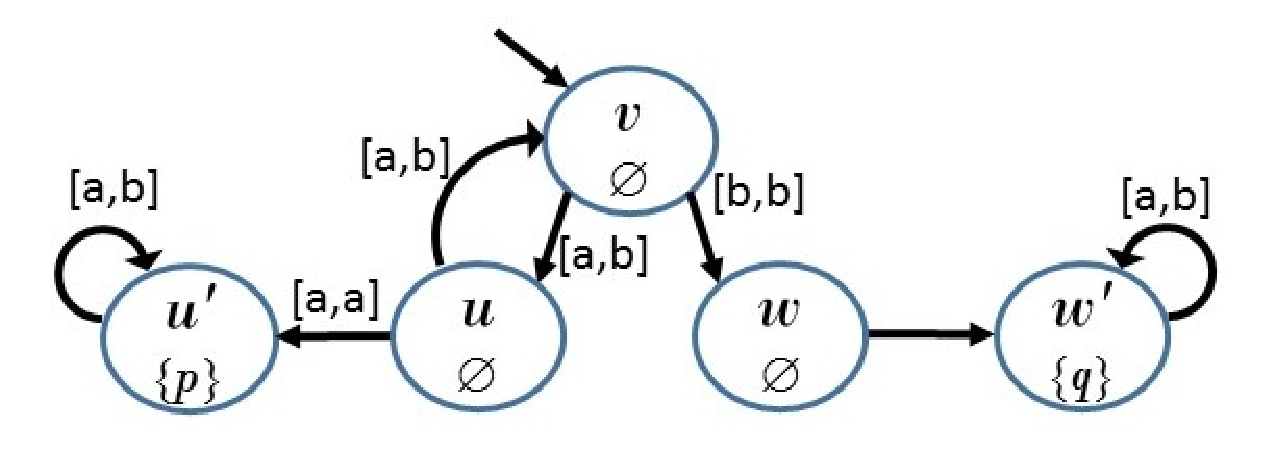
\epsfig{file=cg.eps,width=80mm} 
\end{center}
\caption{A concurrent game graph}
\label{fig.cg}
\end{figure} 
The ovals represent states while the arcs represent 
state transitions.  
We also put down the $\lambda$ values inside the corresponding states. 
On each edge, we label the tokens issued by the agents. 
Specifically, the label on arrow $(q,q')$ is 
$[\delta((q,q'),1),\ldots,\delta((q,q'),m)]$.  
For example, in Figure~\ref{fig.cg}, 
on edge $(v,u)$, we have label $[a,b]$ meaning that 
to make the transition, agent 1 has to choose token $a$ while 
agent 2 has to choose $b$.  




For convenience, in the remaining part of the 
manuscript, we assume that we are always in the context 
of a given game graph
$\calg=\langle m,Q,r,P,\lambda,R,\Delta,\delta\rangle$.
Thus, when we write $Q,r,P,\lambda,R,\Delta$, and $\delta$ 
we respectively refer to the corresponding components of this $\calg$.  



A {\em state predicate} of $P$ is a Boolean combination of elements in $P$.
% We let $\emstp(P)$ be the set of state predicates of $P$.
The satisfaction of a state predicate $\eta$ at a state $q$,
in symbols $q\models \eta$, is defined in the standard way.

A {\em play} is an infinite path in a game graph.
A play is {\em initial} if it begins with the initial state.
Given a play $\rho=\bar{q}_0\bar{q}_1\ldots$,
for every $k\geq 0$, we let $\rho(k)=\bar{q}_k$.
Also, given $h\leq k$,
we let $\rho[h,k]$ denote $\rho(h)\ldots\rho(k)$ and
$\rho[h,\infty)$ denote the infinite tail of $\rho$
from $\rho(h)$.
A {\em play prefix} is a finite segment of a play from the beginning of
the play.
Given a play prefix $\rho=\bar{q}_0\bar{q}_1\ldots \bar{q}_n$, 
we use $|\rho|=n+1$ for the {\em length} of $\rho$.
For convenience, we use $\emlast(\rho)$ to denote the 
last state in $\rho$, i.e., $\rho(|\rho|-1)$.  

Let $Q^*$ be the set of finite sequences of states in $Q$.  
For an agent $a\in [1,m]$,
a {\em strategy} $\sigma$ for $a$ is
a function from $Q^*$ to $\Delta$.
An {\em agency} $A$ of $[1,m]$ is an integer subset of $[1,m]$.  
For example, ``$\{1,3,4\}$'' represents the agency that consists of agents 1, 3, and 4. 
A {\em strategy profile} (or {\em S-profile}) $\Sigma$ of 
an agency $A\subseteq [1,m]$ 
is a partial function from $[1,m]$ to the set of strategies
such that, for every $a\in[1,m]$, 
$a\in A$ iff %\footnote{``{\em iff}" is a shorthand for ``{\em if and only if}."} 
$\Sigma(a)$ is defined.  
The composition of two S-profiles $\Sigma,\Pi$,
in symbols $\Sigma\circ\Pi$, is defined with
the following restrictions for every $a\in[1,m]$.
\begin{list1}
\item If $\Pi(a)$ is defined,
    then $\Sigma\circ\Pi(a)=\Pi(a)$.
\item If $\Sigma(a)$ is defined and $\Pi(a)$ is undefined,
    then $\Sigma\circ\Pi(a)=\Sigma(a)$.
\item If $\Sigma(a)$ and $\Pi(a)$ are both undefined,
    then $\Sigma\circ\Pi(a)$ is also undefined.
\end{list1} 
% Later, w
We will use composition of S-profiles to model 
inheritance of strategy bindings from ancestor formulas. 

A play $\rho$ is compatible with a strategy
$\sigma$ of an agent $a\in [1,m]$
iff for every $k\in [0,\infty)$,
$\delta((\rho(k),\rho(k+1)),a)=\sigma(\rho[0,k])$.
The play is compatible with an S-profile $\Sigma$ of agency $A$
iff for every $a\in A$,
the play is compatible with $\Sigma(a)$ of agent $a$.



\subsection{Turn-based games} 

Another popular game structure is {\em turn-based game} 
in which at each state, at most one agent gets to decide the next state. 
For example, in figure~\ref{fig.tg}, we have the graphical representation of 
a turn-based game graph with initial state $v$.  
\begin{figure}[!ht]
\begin{center}
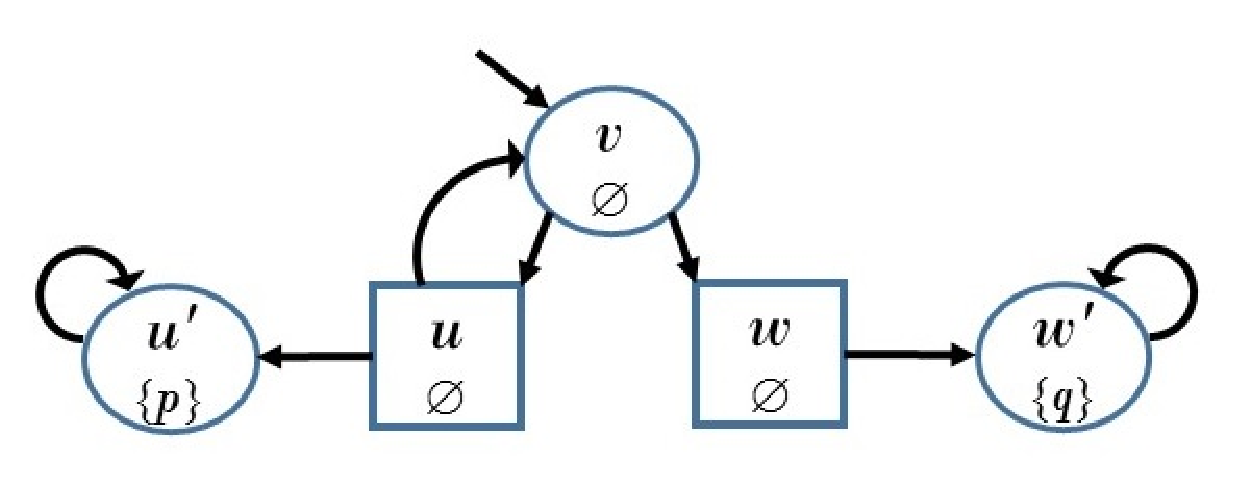
\epsfig{file=tg.eps,width=80mm} \\
$\bigcirc$ belongs to Agent 1 and $\pfrr$ belongs to Agent 2.
\end{center}
\caption{A turn-based game graph}
\label{fig.tg}
\end{figure} 
The ovals and squares represent states respectively of 
agent 1 and agent 2. 
The arcs represent state transitions.  

In fact, every turn-based game can be represented as a special case of 
concurrent games.  
Specifically, a turn-based game 
$\calg=\langle m,Q,r,P,\lambda,E,\Delta,\delta\rangle$ 
can be viewed as a concurrent game with the following restrictions. 
\begin{list1} 
\item $\Delta=Q\cup\{\perp\}$ where $\perp$ denotes a dummy move not in $Q$. 
\item For every $(q,q')\in R$, if $q$ belongs to agent $a$, 
	then $\delta((q,q'),a)=q'$ and 
	for every $a'\neq a$, $\delta((q,q'),a')=\perp$. 
\item For every $(q_1,q_2),(q_3,q_4)\in R$ and agent $a$, 
	$\delta((q_1,q_2),a)=\perp$ if and only if $\delta((q_3,q_4),a)=\perp$.  
	This restriction says that every state can be owned by only one agent. 
\end{list1} 
For convenience, for a turn-based game, 
the owner of a state $q$, $\omega(q)$ in symbols, is defined as agent $a$ with 
$\forall (q,q')\in E(\delta((q,q'),a)=q'$.  
For ease of notation, we denote with 
$Q_a = \{q \in Q \mid \omega(q)=a\}$ 
the states owned by an agent $a$.

In the investigation of many research issues, 
turn-based game graphs are easier to handle than concurrent game graphs.   
So in latter sections, we sometimes use turn-based game graphs 
in examples and explanation of the theory as we see fit. 



\section{Basic Strategy Interaction Logic (BSIL) \label{sec.bsil}} 

\subsection{BSIL syntax \label{subsec.bsil.syntax}}

For concurrent game graph $\calg$ of $m$ agents, 
we have three types of formulas: {\em state formulas}, {\em tree formulas}, 
and {\em path formulas}.  
State formulas describe properties of states.  
Tree formulas describe interaction of strategies.  
Path formulas describe properties of plays.  
BSIL formulas are constructed with the following three syntax rules, 
respectively, for state formulas $\phi$, 
tree formulas $\tau$, and 
path formulas $\theta$.  
\begin{center}
$\begin{array}{rcl}
\phi    & ::= & p\;|\; \neg \phi_1 \;|\; \phi_1\vee \phi_2 
    \;|\; \langle  A\rangle \tau
    \;|\; \langle  A\rangle \theta
    \\
\tau  & ::= & \tau_1\vee \tau_2 \;|\; \tau_1\wedge \tau_2
    \;|\; \langle+ A\rangle \tau_1
    \;|\; \langle+ A\rangle\theta 
    \\
\theta  & ::= & \neg\theta_1 \;|\; \theta_1\vee \theta_2 
    \;|\; \nxt \phi_1
    \;|\; \phi_1\until \phi_2
\end{array}$
\end{center}
Here, $p$ is an atomic proposition in $P$ and
$A$ is an agency of $[1,m]$.
$\langle A\rangle$ is a {\em strategy quantifier} ({\em SQ}) and 
$\langle +A\rangle$ is a {\em strategy interaction quantifier} ({\em SIQ}).  
$\langle A\rangle\psi$ means that
there exists an S-profile for the agency $A$
that makes all plays satisfy $\psi$.
Formulas of the form $\langle+ B\rangle\psi_1$ must happen within an SQ.
Intuitively, they mean that there exists an S-profile of $B$
that collaborates with the strategies declared 
with ancestor formulas to make $\psi_1$ true. 
For convenience, we view SQs as special cases of SIQs. 


State formulas $\phi$ are called {\em BSIL} {\em formulas}. 
From now on, we assume that we are always in the context of 
a given BSIL formula $\chi$.  
Note that we strictly require that strategy interaction cannot 
cross path modal operators.  
This restriction is important and allows us to analyze the interaction 
of strategies locally in a state and 
then enforce the interaction along all paths from this state.  

For convenience, we also use the common shorthands.
\begin{center}
$\begin{array}{rclcrcl}
\true
& \equiv & p\vee(\neg p) 
& \hspace*{10mm} & % \\
\false
& \equiv & \neg\true \\
\psi_1\wedge \psi_2
& \equiv & \neg((\neg\psi_1)\vee(\neg\psi_2)) 
& \hspace*{10mm} & % \\
\psi_1\Rightarrow \psi_2
& \equiv & (\neg \psi_1)\vee \psi_2 \\
\pevt \phi_1
& \equiv & \true\;\until \phi_1 
& \hspace*{10mm} & % \\
\pfrr \phi_1
& \equiv & \neg\pevt\neg\phi_1 \\
\end{array}$
\end{center} 
The SQs and SIQs introduced above are 
all existential in that they are satisfied with one S-profile.  
Note that there is no universal SQs and SIQs in BSIL.  
This is purely for the complexity of the model-checking algorithm (and problem)
that we are going to present later.  
Thus BSIL can be used to specify the different ways of combining S-profiles 
to enforce system policy.  

For ease of notations, 
we may abbreviate 
$\langle \{a_1,\ldots,a_n\}\rangle$ and  
$\langle+ \{a_1,\ldots,a_n\}\rangle$ as 
$\langle a_1,\ldots,a_n\rangle$ and  
$\langle+a_1,\ldots,a_n\rangle$, respectively.




\subsection{BSIL semantics 
\label{subsec.bsil.semantics}}

BSIL subformulas are interpreted with respect to S-profiles.  
A state or a tree formula $\phi$ is satisfied 
at a state $q$ with S-profile $\Sigma$, denoted $\calg,q\models_\Sigma\phi$, if,
and only if, the following inductive constraints are satisfied.
\begin{list1}
\item $\calg,q\models_\Sigma p$ iff $p\in \lambda(q)$.
\item For state formula $\phi_1$, 
    $\calg,q\models_\Sigma\neg\phi_1$ iff
    $\calg,q\models_\Sigma\phi_1$ is false.
\item For state or tree formulas $\psi_1$ and $\psi_2$, 
    $\calg,q\models_\Sigma\psi_1\wedge\psi_2$ iff
    $\calg,q\models_\Sigma\psi_1$
    and $\calg,q\models_\Sigma\psi_2$.
\item For state or tree formulas $\psi_1$ and $\psi_2$, 
    $\calg,q\models_\Sigma\psi_1\vee\psi_2$ iff
    either $\calg,q\models_\Sigma\psi_1$
    or $\calg,q\models_\Sigma\psi_2$.
\item $\calg,q\models_\Sigma\langle A\rangle\tau$
    iff there exists an S-profile $\Pi$ of $A$
    with $\calg,q\models_{\Pi}\tau$.  
\item $\calg,q\models_\Sigma\langle+A\rangle\tau$
    iff there exists an S-profile $\Pi$ of $A$
    with $\calg,q\models_{\Sigma\circ\Pi}\tau$.  
    Here, the composition $\Sigma\circ\Pi$ of the S-profiles $\Sigma$ and $\Pi$
    models the inheritance of 
    strategy bindings, $\Sigma$, from ancestor formulas. 
\item $\calg,q\models_\Sigma\langle A\rangle\theta$
    iff there exists an S-profile $\Pi$ of $A$ such that,
    for all plays $\rho$ from $q$ compatible with $\Pi$,
    $\rho\models_{\Pi}\theta$ holds.
    Intuitively, this means that $\rho$ satisfies path formula $\theta$ with S-profile $\Pi$.  
\item $\calg,q\models_\Sigma\langle + A\rangle\theta$
    iff there exists an S-profile $\Pi$ of $A$ such that, 
    for all plays $\rho$ from $q$ compatible with ${\Sigma\circ\Pi}$,
    $\rho\models_{\Sigma\circ\Pi}\theta$ holds.  
\end{list1} 
% Note that we also let a play $\rho$ satisfy a path formula $\theta$ 
% with the inheritance of an S-profile.  
% This is in fact not necessary for BSIL semantics since 
% all such inheritance will be overruled by SQs immediately.
% However, this is necessary when we later extend BSIL  
% by allowing for the inheritance of strategies across the temporal modal 
% operators.  
%%
%% Commented out, as I don't think we actually do this any more.
%%
A play $\rho$ satisfies a path formula $\theta$ with S-profile $\Sigma$, 
in symbols $\rho\models_\Sigma\theta$, 
iff the following restrictions hold.
\begin{list1} 
\item For a path formula $\theta_1$, 
    $\rho\models_\Sigma\neg\theta_1$ iff
    it is not the case that $\rho\models_\Sigma\theta_1$.
\item For path formulas $\theta_1$ and $\theta_2$, 
    $\rho\models_\Sigma\theta_1\vee\theta_2$ iff
    either $\rho\models_\Sigma\theta_1$
    or $\rho\models_\Sigma\theta_2$.
\item $\rho\models_\Sigma\nxt\psi_1$
    iff $\calg,\rho(1)\models_\Sigma\psi_1$.
\item $\rho\models_\Sigma\psi_1\until\psi_2$
    iff there exists an $h\geq 0$ with $\calg,\rho(h)\models_\Sigma\psi_2$ 
    and for all $j\in [0,h)$, $\calg,\rho(j)\models_\Sigma\psi_1$.
% \item $\rho\models_\Sigma\psi_1\wntil\psi_2$
%     iff either $\rho\models_{\Sigma}\psi_1\until\psi_2$ 
%     or for all $h\geq 0$, $\calg,\rho(h)\models_\Sigma\psi_1$.
%%
%% Commented out, as I don't we did not define W.
%%
\end{list1}
For convenience, we let $\perp$ be a null S-profile, 
i.e., a function that is undefined on everything. 
If $\phi_1$ is a BSIL (state) formula and $\calg,q\models_\perp\phi_1$,
then we may simply write $\calg,q\models\phi_1$.  
If $\calg,r\models\phi_1$, then we also write $\calg\models\phi_1$.  


\subsection{ATL$^+$}
ATL$^+$ is the syntactic fragment of BSIL given by the following grammar

\begin{center}
$\begin{array}{rcl}
\phi    & ::= & p\;|\; \neg \phi_1 \;|\; \phi_1\vee \phi_2 
    \;|\; \langle  A\rangle \theta
    \\
\theta  & ::= & \neg\theta_1 \;|\; \theta_1\vee \theta_2 
    \;|\; \nxt \phi_1
    \;|\; \phi_1\until \phi_2
\end{array}$
\end{center}

ATL$^+$ can also be viewed as an extension of ATL \cite{AHK02} that, similar to ...'s extension of CTL to CTL$^+$ \cite{BPM83,EH86}, allows for the Boolean combination of path formulas.
As such, all complexities of ATL$^+$ must reside between those of BSIL and ATL as well as between those of BSIL and CTL$^+$, which we will use to establish the lower bounds for ATL$^+$ and BSIL.

\subsection{Memory}

In this subsection, we show a simple example that 
the agents need memory to achieve their objective for ATL$^+$ 
specifications.
This is is exemplified by the simplest possible case: 
the turn based game in Figure~\ref{fig.gg.fin} 
with one agent, two states, one atomic proposition, 
and two memoryless strategies 
that do not count the unreached states in the histories.
For the ATL$^+$ sentence 
$\langle 1 \rangle (\langle + \rangle \neg \nxt p) 
\wedge \langle + \rangle \pevt p$, 
apparently agent 1 needs memory to enforce it.  
\begin{figure}[t]
\begin{center} 
\begin{picture}(0,0)%
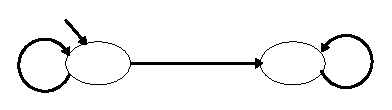
\includegraphics{gg.mem.fin60.eps}%
\end{picture}%
\setlength{\unitlength}{4144sp}%
%
\begingroup\makeatletter\ifx\SetFigFont\undefined%
\gdef\SetFigFont#1#2#3#4#5{%
  \reset@font\fontsize{#1}{#2pt}%
  \fontfamily{#3}\fontseries{#4}\fontshape{#5}%
  \selectfont}%
\fi\endgroup%
\begin{picture}(2724,580)(1631,299)
\put(2197,582){\makebox(0,0)[lb]{\smash{{\SetFigFont{7}{8.4}{\rmdefault}{\mddefault}{\updefault}{\color[rgb]{0,0,0}$v$}%
}}}}
\put(2197,445){\makebox(0,0)[lb]{\smash{{\SetFigFont{7}{8.4}{\rmdefault}{\mddefault}{\updefault}{\color[rgb]{0,0,0}$\emptyset$}%
}}}}
\put(3680,555){\makebox(0,0)[lb]{\smash{{\SetFigFont{7}{8.4}{\rmdefault}{\mddefault}{\updefault}{\color[rgb]{0,0,0}$u$}%
}}}}
\put(3652,418){\makebox(0,0)[lb]{\smash{{\SetFigFont{7}{8.4}{\rmdefault}{\mddefault}{\updefault}{\color[rgb]{0,0,0}$\{p\}$}%
}}}}
\end{picture}%

\end{center}
\caption{A simple turn-based game that demands memoryful strategies}
\label{fig.gg.fin}
\end{figure}

{\lemma \label{lemma.mem.fin}
The strategies of the agents in ATL$^+$ 
(and thus in BSIL) specifications need memory.
This even holds for the single agent case.
\qed 
}


\section{Expressive Power of BSIL \label{sec.exp}}

In this section, we establish that BSIL is incomparable with ATL$^*$, 
AMC, and GL \cite{AHK02} in expressiveness.



\subsection{Comparision with ATL$^*$ \label{subsec.exp.atl} }

It is easy to see that BSIL is a super-class of ATL.
Thus we have the following lemma.

{\lemma \label{lemma.atl.less}
BSIL is at least as expressive as ATL.  
}
% \\\pf The lemma is true since BSIL without SIQs coincides with ATL.  
\qed

Lemmas~\ref{lemma.atl.cant} and \ref{lemma.atl.incomp} establish  
that ATL$^*$ and BSIL are incomparable. 


{\lemma \label{lemma.atl.cant} 
For every ATL$^*$ formula $\phi$,
there are two game graphs that
$\phi$ cannot distinguish while
$\langle 1\rangle ((\langle+ 2\rangle\pfrr p)
    \wedge \langle+ 2\rangle\pfrr q)$ can.
}\\\pf 
The proof is by an inductive construction of 
two families $G_0,\ldots,G_k,\ldots$ 
and $H_0,\ldots,$ $H_k,\ldots$ of turn-based game graphs that 
no ATL$^*$ formula with $k$ SQs can distinguish $G_k$ and $H_k$.  
We prove the lemma by induction on $k$.  

\noindent 
{\bf Base case:} Assume that we have an ATL$^*$ formula 
$\phi$ with at most one SQ.  
Then we have the two game graphs in Figure~\ref{fig.gg.exp}
for three agents.
\begin{figure}[t]\begin{center}
\begin{picture}(0,0)%
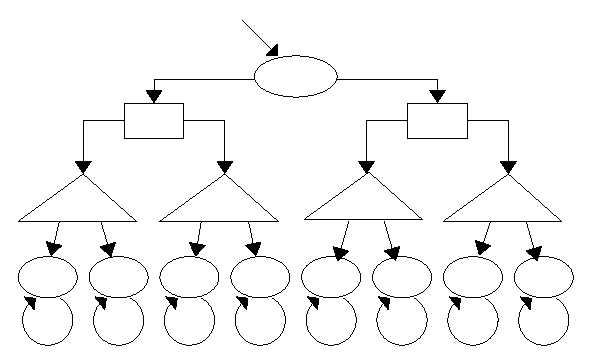
\includegraphics{gg.expba100.eps}%
\end{picture}%
\setlength{\unitlength}{4144sp}%
%
\begingroup\makeatletter\ifx\SetFigFont\undefined%
\gdef\SetFigFont#1#2#3#4#5{%
  \reset@font\fontsize{#1}{#2pt}%
  \fontfamily{#3}\fontseries{#4}\fontshape{#5}%
  \selectfont}%
\fi\endgroup%
\begin{picture}(4250,2496)(169,-1735)
\put(1396,-1276){\makebox(0,0)[lb]{\smash{{\SetFigFont{12}{14.4}{\rmdefault}{\mddefault}{\updefault}{\color[rgb]{0,0,0}$\{q\}$}%
}}}}
\put(3016,-1276){\makebox(0,0)[lb]{\smash{{\SetFigFont{12}{14.4}{\rmdefault}{\mddefault}{\updefault}{\color[rgb]{0,0,0}$\{q\}$}%
}}}}
\put(226,-1276){\makebox(0,0)[lb]{\smash{{\SetFigFont{12}{14.4}{\rmdefault}{\mddefault}{\updefault}{\color[rgb]{0,0,0}$\{p\}$}%
}}}}
\put(2566,-736){\makebox(0,0)[lb]{\smash{{\SetFigFont{12}{14.4}{\rmdefault}{\mddefault}{\updefault}{\color[rgb]{0,0,0}$\{p,q\}$}%
}}}}
\put(3646,-736){\makebox(0,0)[lb]{\smash{{\SetFigFont{12}{14.4}{\rmdefault}{\mddefault}{\updefault}{\color[rgb]{0,0,0}$\{p,q\}$}%
}}}}
\put(1486,-736){\makebox(0,0)[lb]{\smash{{\SetFigFont{12}{14.4}{\rmdefault}{\mddefault}{\updefault}{\color[rgb]{0,0,0}$\{p,q\}$}%
}}}}
\put(406,-736){\makebox(0,0)[lb]{\smash{{\SetFigFont{12}{14.4}{\rmdefault}{\mddefault}{\updefault}{\color[rgb]{0,0,0}$\{p,q\}$}%
}}}}
\put(2071,254){\makebox(0,0)[lb]{\smash{{\SetFigFont{12}{14.4}{\rmdefault}{\mddefault}{\updefault}{\color[rgb]{0,0,0}$\{p,q\}$}%
}}}}
\put(811,-1276){\makebox(0,0)[lb]{\smash{{\SetFigFont{12}{14.4}{\rmdefault}{\mddefault}{\updefault}{\color[rgb]{0,0,0}$\{p\}$}%
}}}}
\put(4051,-1276){\makebox(0,0)[lb]{\smash{{\SetFigFont{12}{14.4}{\rmdefault}{\mddefault}{\updefault}{\color[rgb]{0,0,0}$\{q\}$}%
}}}}
\put(1891,-1276){\makebox(0,0)[lb]{\smash{{\SetFigFont{12}{14.4}{\rmdefault}{\mddefault}{\updefault}{\color[rgb]{0,0,0}$\{q\}$}%
}}}}
\put(2431,-1276){\makebox(0,0)[lb]{\smash{{\SetFigFont{12}{14.4}{\rmdefault}{\mddefault}{\updefault}{\color[rgb]{0,0,0}$\{p\}$}%
}}}}
\put(3511,-1276){\makebox(0,0)[lb]{\smash{{\SetFigFont{12}{14.4}{\rmdefault}{\mddefault}{\updefault}{\color[rgb]{0,0,0}$\{p\}$}%
}}}}
\put(3151,-61){\makebox(0,0)[lb]{\smash{{\SetFigFont{12}{14.4}{\rmdefault}{\mddefault}{\updefault}{\color[rgb]{0,0,0}$\{p,q\}$}%
}}}}
\put(991,-61){\makebox(0,0)[lb]{\smash{{\SetFigFont{12}{14.4}{\rmdefault}{\mddefault}{\updefault}{\color[rgb]{0,0,0}$\{p,q\}$}%
}}}}
\put(2341,524){\makebox(0,0)[lb]{\smash{{\SetFigFont{12}{14.4}{\rmdefault}{\mddefault}{\updefault}{\color[rgb]{0,0,0}$r_0$}%
}}}}
\end{picture}%
\\
(a) $G_0$, a game graph for base case.\\
\begin{picture}(0,0)%
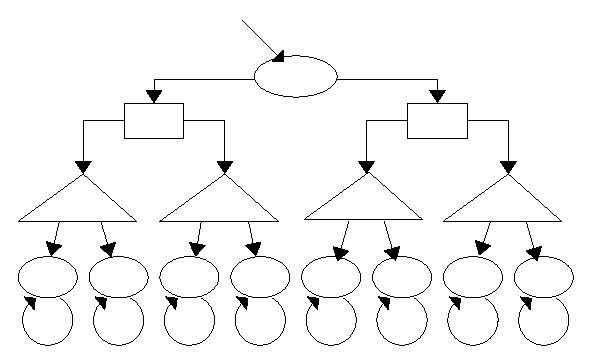
\includegraphics{gg.expbb100.eps}%
\end{picture}%
\setlength{\unitlength}{4144sp}%
%
\begingroup\makeatletter\ifx\SetFigFont\undefined%
\gdef\SetFigFont#1#2#3#4#5{%
  \reset@font\fontsize{#1}{#2pt}%
  \fontfamily{#3}\fontseries{#4}\fontshape{#5}%
  \selectfont}%
\fi\endgroup%
\begin{picture}(4250,2496)(169,-1735)
\put(856,-1276){\makebox(0,0)[lb]{\smash{{\SetFigFont{12}{14.4}{\rmdefault}{\mddefault}{\updefault}{\color[rgb]{0,0,0}$\{p\}$}%
}}}}
\put(1396,-1276){\makebox(0,0)[lb]{\smash{{\SetFigFont{12}{14.4}{\rmdefault}{\mddefault}{\updefault}{\color[rgb]{0,0,0}$\{p\}$}%
}}}}
\put(3016,-1276){\makebox(0,0)[lb]{\smash{{\SetFigFont{12}{14.4}{\rmdefault}{\mddefault}{\updefault}{\color[rgb]{0,0,0}$\{q\}$}%
}}}}
\put(3556,-1276){\makebox(0,0)[lb]{\smash{{\SetFigFont{12}{14.4}{\rmdefault}{\mddefault}{\updefault}{\color[rgb]{0,0,0}$\{p\}$}%
}}}}
\put(226,-1276){\makebox(0,0)[lb]{\smash{{\SetFigFont{12}{14.4}{\rmdefault}{\mddefault}{\updefault}{\color[rgb]{0,0,0}$\{p\}$}%
}}}}
\put(2566,-736){\makebox(0,0)[lb]{\smash{{\SetFigFont{12}{14.4}{\rmdefault}{\mddefault}{\updefault}{\color[rgb]{0,0,0}$\{p,q\}$}%
}}}}
\put(3646,-736){\makebox(0,0)[lb]{\smash{{\SetFigFont{12}{14.4}{\rmdefault}{\mddefault}{\updefault}{\color[rgb]{0,0,0}$\{p,q\}$}%
}}}}
\put(1486,-736){\makebox(0,0)[lb]{\smash{{\SetFigFont{12}{14.4}{\rmdefault}{\mddefault}{\updefault}{\color[rgb]{0,0,0}$\{p,q\}$}%
}}}}
\put(406,-736){\makebox(0,0)[lb]{\smash{{\SetFigFont{12}{14.4}{\rmdefault}{\mddefault}{\updefault}{\color[rgb]{0,0,0}$\{p,q\}$}%
}}}}
\put(2071,254){\makebox(0,0)[lb]{\smash{{\SetFigFont{12}{14.4}{\rmdefault}{\mddefault}{\updefault}{\color[rgb]{0,0,0}$\{p,q\}$}%
}}}}
\put(4051,-1276){\makebox(0,0)[lb]{\smash{{\SetFigFont{12}{14.4}{\rmdefault}{\mddefault}{\updefault}{\color[rgb]{0,0,0}$\{q\}$}%
}}}}
\put(3151,-106){\makebox(0,0)[lb]{\smash{{\SetFigFont{12}{14.4}{\rmdefault}{\mddefault}{\updefault}{\color[rgb]{0,0,0}$\{p,q\}$}%
}}}}
\put(991,-106){\makebox(0,0)[lb]{\smash{{\SetFigFont{12}{14.4}{\rmdefault}{\mddefault}{\updefault}{\color[rgb]{0,0,0}$\{p,q\}$}%
}}}}
\put(1891,-1276){\makebox(0,0)[lb]{\smash{{\SetFigFont{12}{14.4}{\rmdefault}{\mddefault}{\updefault}{\color[rgb]{0,0,0}$\{q\}$}%
}}}}
\put(2431,-1276){\makebox(0,0)[lb]{\smash{{\SetFigFont{12}{14.4}{\rmdefault}{\mddefault}{\updefault}{\color[rgb]{0,0,0}$\{q\}$}%
}}}}
\put(2296,524){\makebox(0,0)[lb]{\smash{{\SetFigFont{12}{14.4}{\rmdefault}{\mddefault}{\updefault}{\color[rgb]{0,0,0}$s_0$}%
}}}}
\end{picture}%
\\
(b) $H_0$, another game graph for base case.\\
$\bigcirc$ belongs to Agent  1; $\pfrr$ belongs to Agent 2; and 
$\triangle$ belongs to Agent 3.
\end{center}
\caption{Base cases for the expressiveness of BSIL over ATL$^*$}
\label{fig.gg.exp}
\end{figure}
Note that the two game graphs have the same set of traces.
Thus they cannot be distinguished by path formulas.
Then there are the following case analysis of ATL$^*$ formulas.
\begin{list1}
\item {\bf Case 1:} {\em $\phi$ is $\langle A\rangle\phi_1$
    where $\phi_1$ is a Boolean combination of path formulas.}
    Note that $\phi_1$ characterizes a set of traces.
    For convenience of discussion,
    we call a trace that stabilizes to $\{p\}$ a $p$-trace.
    A trace that stabilizes to $\{q\}$ is called a $q$-trace.
    Also, for a path formula $\theta$,
    we let $\ldbrac\theta\rdbrac$ denote the
    set of traces characterized by $\theta$.
    For the two game graphs in figure~\ref{fig.gg.exp},
    there are only two types of traces.
    Thus there are only the following
    four different subsets of traces.
    \begin{list1}
    \item The set of no trace, denoted $\emptyset$.
    \item The set of $p$-traces, denoted $\{\pfrr p\}$.
    \item The set of $q$-traces, denoted $\{\pfrr q\}$.
    \item The set of $p$-traces and $q$-traces,
        denoted $\{\pfrr p,\pfrr q\}$.
    \end{list1}
    The following case analysis shows that, for every
    trace subset $S$ and every agency $A$,
    there exists a strategy of $A$ to characterize
    $S$ in figure~\ref{fig.gg.exp}(a) iff
    there exists a strategy for $A$ to characterize
    $S$ in figure~\ref{fig.gg.exp}(b).
    \begin{list2}
    \item {\bf Case 1a:} {\em $\phi$ is $\langle\emptyset\rangle\phi_1$.}
        In this case, there is no strategy and the sets of traces
        imposed by no strategy in the two state graphs are
        both $\{\pfrr p,\pfrr q\}$.
        Thus, $\langle\emptyset\rangle\phi_1$ cannot distinguish the trace sets of the
        two state graphs.
    \item {\bf Case 1b:} {\em $\phi$ is $\langle 1\rangle\phi_1$.}
        From figure~\ref{fig.gg.exp}, no matter what strategies
        agency $\{1\}$ may choose, the
        trace sets for the two game graphs are both
        $\{\pfrr p,\pfrr q\}$.
        Thus, $\langle 1\rangle\phi_1$ cannot distinguish the trace sets of the
        two state graphs.
    \item {\bf Case 1c:} {\em $\phi$ is
        $\langle 2\rangle\phi_1$.}
        This case is similar to case 1b.
    \item {\bf Case 1d:} {\em $\phi$ is
        $\langle 3\rangle\phi_1$.}
        This case is similar to case 1b.
    \item {\bf Case 1e:} {\em $\phi$ is
        $\langle 1,2\rangle\phi_1$.}
        Agency $\{1, 2\}$ can cooperate to force three trace sets:
        $\{\pfrr p\}, \{\pfrr q\}, \{\pfrr p,\pfrr q\}$
        in both of the game graphs in figure~\ref{fig.gg.exp}.
        Thus, $\langle 1,2\rangle\phi_1$ cannot distinguish the trace sets of the
        two state graphs.
    \item {\bf Case 1f:} {\em $\phi$ is
        $\langle 1,3\rangle\phi_1$.}
        This case is similar to case 1e.
    \item {\bf Case 1g:} {\em $\phi$ is
        $\langle 2,3\rangle\phi_1$.}
        This case is similar to case 1e.
    \item {\bf Case 1h:} {\em $\phi$ is
        $\langle 1,2,3\rangle\phi_1$.}
        Agency $\{1, 2,3\}$ can cooperate to force three trace sets:
        $\{\pfrr p\}, \{\pfrr q\}, \{\pfrr p,\pfrr q\}$
        in both of the game graphs in figure~\ref{fig.gg.exp}.
        Thus, $\langle 1,2,3\rangle\phi_1$ cannot distinguish the trace sets of the
        two state graphs.
    \end{list2}
\item {\bf Case 2:} {\em $\phi$ is a Boolean combination of
    formulas in case 1.}
    Since case 1 does not distinguish the two game graphs,
    this case can neither do it.
\end{list1}
Thus the base case is proven.

\noindent {\bf Induction step:}
We use structural induction on ATL$^*$ formulas to prove the step.
If $\phi$ has $k$ SQs,
then we can construct the two graphs in figure~\ref{fig.gg.expi}.
\begin{figure}[t]\begin{center}
\begin{picture}(0,0)%
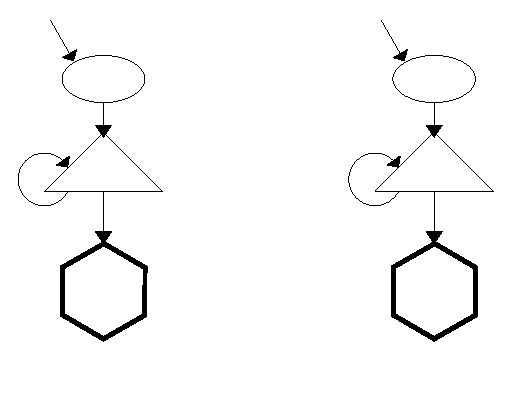
\includegraphics{gg.expi100.eps}%
\end{picture}%
\setlength{\unitlength}{4144sp}%
%
\begingroup\makeatletter\ifx\SetFigFont\undefined%
\gdef\SetFigFont#1#2#3#4#5{%
  \reset@font\fontsize{#1}{#2pt}%
  \fontfamily{#3}\fontseries{#4}\fontshape{#5}%
  \selectfont}%
\fi\endgroup%
\begin{picture}(3643,2925)(1635,-2164)
\put(1891,-2086){\makebox(0,0)[lb]{\smash{{\SetFigFont{12}{14.4}{\rmdefault}{\mddefault}{\updefault}{\color[rgb]{0,0,0}(a) $G_k$}%
}}}}
\put(4411,-2086){\makebox(0,0)[lb]{\smash{{\SetFigFont{12}{14.4}{\rmdefault}{\mddefault}{\updefault}{\color[rgb]{0,0,0}(b) $H_k$}%
}}}}
\put(2116,-1366){\makebox(0,0)[lb]{\smash{{\SetFigFont{12}{14.4}{\rmdefault}{\mddefault}{\updefault}{\color[rgb]{0,0,0}$G_{k-1}$}%
}}}}
\put(4636,-1366){\makebox(0,0)[lb]{\smash{{\SetFigFont{12}{14.4}{\rmdefault}{\mddefault}{\updefault}{\color[rgb]{0,0,0}$H_{k-1}$}%
}}}}
\put(2071,-466){\makebox(0,0)[lb]{\smash{{\SetFigFont{12}{14.4}{\rmdefault}{\mddefault}{\updefault}{\color[rgb]{0,0,0}$\{p,q\}$}%
}}}}
\put(4591,-466){\makebox(0,0)[lb]{\smash{{\SetFigFont{12}{14.4}{\rmdefault}{\mddefault}{\updefault}{\color[rgb]{0,0,0}$\{p,q\}$}%
}}}}
\put(4591,254){\makebox(0,0)[lb]{\smash{{\SetFigFont{12}{14.4}{\rmdefault}{\mddefault}{\updefault}{\color[rgb]{0,0,0}$\{p,q\}$}%
}}}}
\put(2071,254){\makebox(0,0)[lb]{\smash{{\SetFigFont{12}{14.4}{\rmdefault}{\mddefault}{\updefault}{\color[rgb]{0,0,0}$\{p,q\}$}%
}}}}
\put(2251,524){\makebox(0,0)[lb]{\smash{{\SetFigFont{12}{14.4}{\rmdefault}{\mddefault}{\updefault}{\color[rgb]{0,0,0}$r_k$}%
}}}}
\put(4816,524){\makebox(0,0)[lb]{\smash{{\SetFigFont{12}{14.4}{\rmdefault}{\mddefault}{\updefault}{\color[rgb]{0,0,0}$s_k$}%
}}}}
\end{picture}%
\\
$\bigcirc$ belongs to Agent  1; $\pfrr$ belongs to Agent 2; and 
$\triangle$ belongs to Agent 3.
\end{center}
\caption{Inductive cases for the expressiveness of BSIL over ATL$^*$}
\label{fig.gg.expi}
\end{figure}
It is clear that
$\langle 1\rangle ((\langle+ 2\rangle \pfrr p)
    \wedge (\langle+ 2\rangle \pfrr q))$ can distinguish
$G_k$ and $H_k$.
However, to tell the difference between the two graphs,
we need a modal subformula of $\phi$ that can tell the difference
of $G_{k-1}$ and $H_{k-1}$.
But according to the inductive hypothesis, this is impossible.
Thus the lemma is proven.  
\qed 

Lemmas~\ref{lemma.atl.less} and \ref{lemma.atl.cant} together establish  
that ATL is strictly less expressive than BSIL. 


{\lemma \label{lemma.atl.incomp}
ATL$^*$ formula $\langle 1\rangle\pfrr\pevt p$
is not equivalent to any BSIL formula.
} 
\\\pf 
The proof is similar to the proof for the inexpressibility of 
$\langle 1\rangle\pfrr\pevt p$ with ATL \cite{AHK02}.  
\qed 

Lemmas~\ref{lemma.atl.cant} and \ref{lemma.atl.incomp}
together establish  
that ATL$^*$ and BSIL are not comparable in expressiveness. 





\subsection{Comparision with GL\label{subsec.exp.gl}} 

GL separates strategy quantificaitons from path quantifications.  
In comparison, ATL$^*$ and BSIL combines these two quantifications 
into SQs and SIQs.  
Thus with GL, we can specify that, for all S-profiles of $A$, 
there exists a play saitsfying $\psi_1$.  
The (existential) strategy quantification for agency $A$ 
of GL is of the form $\existsb A.\psi_1$.  
The path quantifications are just ordinary CTL modalities: 
$\forall\pfrr, \forall\until, \exists\pfrr$, and 
$\exists\until$.  

The following two lemmas show the relation between GL and BSIL.  

{\lemma \label{lemma.gl.cant}
For every GL formula $\phi$,
there are two game graphs that
$\phi$ cannot distinguish while \linebreak 
$\langle 1\rangle ((\langle+ 2\rangle\pfrr p)
    \wedge \langle+ 2\rangle\pfrr q)$ can.
}
\\\pf 
The proof is similar to the one for Lemma~\ref{lemma.atl.cant} 
and is by induction on the number of modal operators $k$.  

\noindent 
{\bf Base case:} Assume that $\phi$ has only one modal operator.
Then we have the two game graphs in figure~\ref{fig.gg.exp}
for three agents.
Then there are the following case analysis of GL formulas.
\begin{list1}
\item {\bf Case 1:} {\em $\phi$ is $\existsb  A.\phi_1$
    where $\phi_1$ is a Boolean combination of
    formulas of the form $\exists \psi$ or $\forall \psi$
    where $\psi$ is a path formula.}
    Note that $\phi_1$ characterizes a set of states that 
    either start a play satisfying $\psi$ or 
    start only plays satisfying $\psi$.
    The following case analysis shows that, for every
    trace subset $S$ and every agency $A$,
    there exists a strategy of $A$ to characterize
    $S$ in figure~\ref{fig.gg.exp}(a) iff
    there exists a strategy for $A$ to characterize
    $S$ in figure~\ref{fig.gg.exp}(b).
    \begin{list2}
    \item {\bf Case 1a:} {\em $\phi$ is $\existsb\emptyset.\phi_1$.}
        In this case, there is no strategy and the sets of traces
        imposed by no strategy in the two state graphs are
        both $\{\pfrr p,\pfrr q\}$.
        Thus, $\existsb\emptyset.\phi_1$ cannot distinguish the trace sets of the
        two state graphs.
    \item {\bf Case 1b:} {\em $\phi$ is $\existsb\{1\}.\phi_1$.}
        From figure~\ref{fig.gg.exp}, no matter what strategies
        agency $\{1\}$ may choose, the
        trace sets for the two game graphs are both
        $\{\pfrr p,\pfrr q\}$.
        Thus, $\existsb\{1\}.\phi_1$ cannot distinguish the trace sets of the
        two state graphs.
    \item {\bf Case 1c:} {\em $\phi$ is
        $\existsb\{2\}.\phi_1$.}
        This case is similar to case 1b.
    \item {\bf Case 1d:} {\em $\phi$ is
        $\existsb\{3\}.\phi_1$.}
        This case is similar to case 1b.
    \item {\bf Case 1e:} {\em $\phi$ is
        $\existsb\{1,2\}.\phi_1$.}
        Agency $\{1, 2\}$ can cooperate to force three trace sets:
        $\{\pfrr p\}, \{\pfrr q\}, \{\pfrr p,\pfrr q\}$
        in both of the game graphs in figure~\ref{fig.gg.exp}.
        Thus, $\existsb\{1,2\}.\phi_1$ cannot distinguish the trace sets of the
        two state graphs.
    \item {\bf Case 1f:} {\em $\phi$ is
        $\existsb\{1,3\}.\phi_1$.}
        This case is similar to case 1e.
    \item {\bf Case 1g:} {\em $\phi$ is
        $\existsb\{2,3\}.\phi_1$.}
        This case is similar to case 1e.
    \item {\bf Case 1h:} {\em $\phi$ is
        $\existsb\{1,2,3\}.\phi_1$.}
        Agency $\{1, 2,3\}$ can cooperate to force three trace sets:
        $\{\pfrr p\}, \{\pfrr q\}, \{\pfrr p,\pfrr q\}$
        in both of the game graphs in figure~\ref{fig.gg.exp}.
        Thus, $\existsb\{1,2,3\}.\phi_1$ cannot distinguish the trace sets of the
        two state graphs.
    \end{list2}
\item {\bf Case 2:} {\em $\phi$ is a Boolean combination of
    formulas in case 1.}
    Since case 1 does not distinguish the two game graphs, 
    this case can neither do it.  
\end{list1}
Thus the base case is proven.

\noindent {\bf Induction step:}
We use structural induction on GL formulas to prove the step.
If $\phi$ has $k$ modal operators,
then we can use the two graphs in figure~\ref{fig.gg.expi}.
It is clear that
$\langle 1\rangle ((\langle+ 2\rangle \pfrr p)
    \wedge (\langle+ 2\rangle \pfrr q))$ can distinguish
the two graphs.
However, to tell the difference between the two graphs,
we need a modal subformula of $\phi$ that can tell the difference
of $G_{k-1}$ and $H_{k-1}$.
But according to the inductive hypothesis, this is impossible.
Thus the lemma is proven.  
\qed 



{\lemma \label{lemma.gl.incomp}
GL formula $\existsb\{1\}.((\exists\pfrr p)\wedge\exists\pfrr q)$
is not equivalent to any BSIL formula.
}
\\\pf The proof basically follows the same argument in \cite{AHK02} 
that $\existsb\{1\}.((\exists\pfrr p)\wedge\exists\pfrr q)$ 
is not equivalent to 
any ATL$^*$ formula.  
\qed 

Lemmas~\ref{lemma.gl.cant} and 
\ref{lemma.gl.incomp} together show that 
GL and BSIL are not comparable in expressiveness.  






\subsection{Comparision with AMC\label{subsec.exp.amc}} 

AMC is an extension from $\mu$-calculus and allows 
for multiple fixpoints interleaved together \cite{AHK02}.  
An AMC formula contains fixpoint operators on state set variables.  
The only modality of AMC is of the form $\langle A\rangle\nxt\psi$ 
and least fixpoint $\emlfp x.\psi_1(x)$ where 
$\psi_1(x)$ is a Boolean function of atomic propositions 
and state set variables (including $x$).  
It is required that every occurrence of $x$ in $\psi_1$ is 
under even number of negations.  
The duality of the least fixpoint operator is the greatest fixpoint 
operator $\emgfp$.  
Formula $\emgfp x.\psi_1$ is defined as $\neg\emlfp x.\neg\psi_1(x)$.  

To establish that AMC is not as expressive as BSIL, we basically follow 
the proof style for Lemma~\ref{lemma.atl.cant} and 
use the same two families of game graphs.  
% (See appendix~\ref{app.lemma.atl.cant}).  
The statement of the lemma requires notations for 
state set variables and other details in AMC. 
We need to define the domain of values for the free state set variables 
in AMC formulas.  
Let $X$ be the set of state set variables.  
Without loss of generality, we assume that no two subformulas
of the form $\emlfp x.\phi$ in
a given AMC formula share the same quantified name of $x$.
Given a subformula $\emlfp x_i.\phi$
with free variables $x_1,\ldots,x_n$ in $\phi$
and no modal operator $\langle\ldots\rangle\nxt$ in $\phi$,
we define $\phi$ as a {\em base template} for $x_i$.
Then we can define the {\em base formula domain} of $x_i$,
denoted $F_0(x_i)$,
as the smallest set with the following restrictions.
We let $\phi[x_1\mapsto \eta_1,\ldots,x_n\mapsto\eta_n]$ 
be the AMC formula identical to 
$\phi$ except that every occurrence of $x_i$ in $\phi$ are respectively 
replaced with $\eta_i$.  
\begin{list1}
\item For each $x_i\in X$ with base template $\phi$,
    $\phi[x_1\mapsto\false,\ldots,x_n\mapsto\false]\in F_0(x_i)$.
\item For each $x_i\in X$ with base template $\phi$
    and $\phi_1\in F_0(x_1),\ldots,\phi_n\in F_0(x_n)$,
    $\phi[x_1\mapsto\phi_1,\ldots,x_n\mapsto\phi_n]\in F_0(x_i)$.
\end{list1}
Note that there is neither variables nor `$\emlfp$' operators
in $F_0(x)$ for every $x$.
Thus we can define the characterization $\kappa$ 
of a formula $\phi_1$ in $F_0(x)$ for $\calg$,
in symbols $\kappa(\calg,\phi_1)$, as follows.
\begin{list1}
\item For each atomic proposition $p\in P$,
    $\kappa(\calg,p)=\{q\mid p\in\lambda(q)\}$.
\item For each $\phi\in F_0(x)$, 
    $\kappa(\calg,\neg\phi)=Q-\kappa(\calg,\phi)$.
\item For each $\phi_1,\phi_2\in F_0(x)$,
    $\kappa(\calg,\phi_1\vee\phi_2)=\kappa(\calg,\phi_1)\cup\kappa(\calg,\phi_2)$.
\end{list1}
A {\em valuation} $\nu$ of variables in $X$ for $\calg$
is a mapping from
$X$ such that, for each $x\in X$, there exists a base domain formula
$\phi$ of $x$ such that $\nu(x)= \kappa(\calg,\phi)$.

The expressiveness comparison between AMC and BSIL relies on the
following lemma.

{\lemma \label{lemma.amc.domain}
For every AMC formula $\phi$ without modal operator of the
form $\langle\ldots\rangle\nxt$, state set variable $x$, and
a formula $\phi_1$ in $F_0(x)$,
$r_0\in\kappa(G_0,\phi_1)$
iff
$s_0\in\kappa(H_0,\phi_1)$
in figure~\ref{fig.gg.exp}.
}
\\\pf 
We can prove this with an structural induction on $\phi_1$.
The base case is straightforward.
The inductive step follows since Boolean combinations of
subformulas that cannot distinguish $G_0$ and $H_0$ can neither
distinguish the two game graphs.
\qed





Now we want to classify AMC formulas according to the nesting depths of
operators of the form $\langle\ldots\rangle\nxt$ in a formula.
Specifically, we let $\mbox{AMC}^{(k)}$ be the set of AMC formulas
with exactly nesting depth $k$ of operator $\langle \ldots\rangle\nxt$.
For example,
$\emlfp x.\langle 1\rangle \nxt
(p\rightarrow \emlfp y.\langle 2\rangle (x\vee y\wedge\nxt q))$
is in $\mbox{AMC}^{(2)}$.
Then, $\mbox{AMC}^{(0)}$ is
the smallest set with the following restrictions.
\begin{list1}
\item {\bf Case 1a:} For each atomic proposition $p\in P$,
    $p\in \mbox{AMC}^{(0)}$.
\item {\bf Case 1b:} For each proposition variable $x\in X$,
    $x\in \mbox{AMC}^{(0)}$.
\item {\bf Case 1c:} For each $\phi\in \mbox{AMC}^{(0)}$,
    $\neg\phi\in \mbox{AMC}^{(0)}$.
\item {\bf Case 1d:} For each $\phi_1,\phi_2\in \mbox{AMC}^{(0)}$,
    $\phi_1\vee\phi_2\in \mbox{AMC}^{(0)}$.
\item {\bf Case 1e:} For each $\phi\in \mbox{AMC}^{(0)}$ and
    proposition variable $x\in X$,
    $\emlfp x.\phi\in \mbox{AMC}^{(0)}$.
\end{list1}
Then $\mbox{AMC}^{(k)}$, $k>0$,
is the smallest set with the following restrictions.
\begin{list1}
\item {\bf Case 2a:} For each $A\subseteq [1,m]$ and
    $\phi\in \mbox{AMC}^{(k-1)}$,
    $\langle A\rangle \nxt \phi\in \mbox{AMC}^{(k)}$,
\item {\bf Case 2b:} For each $\phi\in \mbox{AMC}^{(k)}$,
    $\neg\phi\in \mbox{AMC}^{(k)}$.
\item {\bf Case 2c:} For each $\phi_1\in \mbox{AMC}^{(k)}$ and
    $\phi_2\in\bigcup_{h\leq k}\mbox{AMC}^{(h)}$,
    $\phi_1\vee\phi_2\in \mbox{AMC}^{(k)}$.
\item {\bf Case 2d:} For each
    $\phi_1\in\bigcup_{h\leq k}\mbox{AMC}^{(h)}$ and $\phi_2\in \mbox{AMC}^{(k)}$,
    $\phi_1\vee\phi_2\in \mbox{AMC}^{(k)}$.
\item {\bf Case 2e:} For each $\phi\in \mbox{AMC}^{(k)}$ and
    proposition variable $x\in X$,
    $\emlfp x.\phi\in \mbox{AMC}^{(k)}$.
\end{list1}
Note that there could be free variables in the formulas classified in
the above.
The evaluation of such formulas for a game graph depends on the
valuation of the free variables.

Given two game graphs $G,H$ and
an AMC formulas $\phi$,
we say that
two valuations of $\nu$ and $\nu'$ respectively of $G$ and $H$
are {\em consistent} if for every $x\in X$,
there exists a $\phi_1\in F_0(x)$ such that
$\nu(x)=\kappa(G,\phi_1)$ and $\nu'(x)=\kappa(H,\phi_1)$.
In the following, we adopt the AMC semantic notations in \cite{AHK02}.
Given a game graph $G$, an AMC formula $\phi$,
and a valuation $\nu$ of state set variables in $X$,
$(\phi)^G(\nu)$ denotes the set of states of $G$ that
satisfy $\phi$ with valuation $\nu$.







{\lemma\label{lemma.amc.induction}
Assume that $G_k$ and $H_k$ are defined in
figures~\ref{fig.gg.exp} and \ref{fig.gg.expi}.
For every $k$, AMC formula $\phi\in \mbox{AMC}^{(k)}$, and two consistent
valuations $\nu$ and $\nu'$ respectively of $G_k$ and $H_k$,
$r_k\in (\phi)^{G_k}(\nu)$ iff
$s_k\in (\phi)^{H_k}(\nu')$.
}
\\\pf
We use an induction on $k$ to prove the lemma.

\noindent
{\bf Base case:} 
When $\phi$ is in case 1a through 1d, the lemma follows straightforwardly.
In case 1e,
$(\emlfp x.\psi)^{G_0}(\nu)$ can be expanded as follows.
We let
\begin{list1}
\item $\psi^{G_0,\nu,(0)}$ be $(\psi[x\mapsto \false])^{G_0}(\nu)$ and
\item for each $h>0$,
    $\psi^{G_0,\nu,(h)}$ be $(\phi[x\mapsto \psi_1^{G_0,(h-1)}])(\nu)$.
\end{list1}
Then $(\emlfp x.\phi)^{G_0}(\nu)=\bigcup_{h\geq 0}\psi^{G_0,\nu,(h)}$
according to the semantics of AMC.
Similarly, \linebreak 
$(\emlfp x.\phi)^{H_0}(\nu')=\bigcup_{h\geq 0}\psi^{H_0,\nu',(h)}$.
According to the same argument for cases 1a through 1d,
for each $h\geq 0$,
$r_0\in \psi^{G_0,\nu,(h)}$ iff
$s_0\in \psi^{H_0,\nu',(h)}$.
Thus it is clear that
$r_0\in (\emlfp x.\phi)^{G_0}(\nu)$ iff
$s_0\in (\emlfp x.\phi)^{H_0}(\nu')$.
Thus the lemma is proven in this case.

\noindent
{\bf Induction step:}
To tell the difference between $G_k$ and $H_k$,
we need a formula with the following structure.
\begin{list1}
\item At least one nesting of operators
    like $\langle\ldots\rangle\nxt$ in a least fixpoint operation 
    to infer the reachability of $G_{k-1}$ and $H_{k-1}$.
\item A modal subformula nested inside a $\langle \ldots\rangle \nxt$
    modal operator of $\phi$ that can tell the difference
    of $G_{k-1}$ and $H_{k-1}$.  
    But according to the inductive hypothesis, this is impossible.  
\end{list1}
Thus the lemma is proven.
\qed


Then with Lemma~\ref{lemma.amc.induction}, 
we conclude the proof for Lemma~\ref{lemma.amc.cant} in the following. 


{\lemma \label{lemma.amc.cant}
For every AMC formula $\phi$,
there are two game graphs that
$\phi$ cannot distinguish while
$\langle 1\rangle ((\langle+ 2\rangle\pfrr p)
    \wedge \langle+ 2\rangle\pfrr q)$ can.
}
\\\pf 
In the proof for Lemma~\ref{lemma.amc.induction}, 
it is apparent that $\phi$ with $\phi\in\mbox{AMC}^{(k)}$ cannot 
tell $G_k$ and $H_k$.  
\qed 

By the same argument in \cite{AHK02}, 
for one-agent game, BSIL coincides with CTL and is not as expressive as 
AMC. 

{\lemma \label{lemma.amc.can}
For game graphs of one agent,
AMC is strictly more expressive than BSIL.} 
\\\pf 
For one-agent games, 
AMC is equivalent to $\mu$-calculus and BSIL is equivalent to CTL which
is strictly less expressive than $\mu$-calculus.
\qed 



A comment on Lemmas~\ref{lemma.atl.cant}, 
\ref{lemma.gl.cant}, and \ref{lemma.amc.cant} 
is that the path modal formulas in the lemmas can be changed 
independently to $\pevt \neg p$ and $\pevt \neg q$ without affecting the validity of 
the lemma.  
This can be used to show that the example properties in the introduction 
are indeed inexpressible in ATL$^*$, GL, and AMC.  




\section{BSIL and ATL$^+$ model-checking are PSPACE complete 
\label{sec.mck.psp}}





The model-checking problem of BSIL is contained in 
PSPACE mainly due to the restriction that disallows 
negation in tree formulas.
As in the model-checking algorithms 
of ATL \cite{AHK02}, we can evaluate the proper state subformulas  
formulas independently and then treat them as auxiliary propositions.  
Moreover, as in the evaluation of $\pevt$-formulas in 
ATL model-checking, 
if a $\pevt$-formula can be enforced with an S-profile, it can be enforced 
in a finite number of steps along every play compatible with 
the strategy in a computation tree.  
Once a bound $b$ for this finite number of steps is determined, 
we can enumerate all strategies embedded in the computation 
tree up to depth $b$ and try to find one that enforces a BSIL formula.  

There are, however, severe differences between exploring 
a computation tree for 
BSIL and exploring one for ATL \cite{AHK02}.   
For BSIL, we have to take the interaction of strategies into account.  
For example, we may have to enforce a subformula 
$\langle 1\rangle((\langle+ 2\rangle \pevt p)
\wedge\langle+ 2\rangle (\pfrr q\vee \pevt r))$.  
Then, when exploring the computation tree, 
we may follow two strategies of Agent 2, one to enforce $\pevt p$ and 
the other to enforce $\pfrr q$ or $\pevt r$.  
There are the following situation for the 
interaction between these two strategies. 
The two strategies may make the same decision all the way 
until we reach a tree node $v$.  
(For turn-based games, $v$ has to be owned by Agent 2.)    
This can be conceptualized as passing the obligations of $\pevt p$ and 
$\pfrr q\vee\pevt r$ along the path from the root to $v$.  
Then, at node $v$, the two strategies may differ in their decisions 
and pass down the two obligations to different branches. 
In Subsection~\ref{subsec.children.ltl.ob},
we explain some basic concepts in labeling the children with
path obligations passed down from their parent in a computation tree
to obey the interaction among the strategies declared in a BSIL formula.

Then, in Subsection~\ref{subsec.alg.proc},
we present our algorithm in two parts,
one for model-checking BSIL state formulas
and the other for model-checking BSIL tree formulas.
In Subsection~\ref{subsec.alg.corr},
we prove the correctness of the algorithm.
In Subsection~\ref{subsec.alg.pspace}, 
we show that our algorithm is in PSPACE.  
Together with Lemma~\ref{lemma.bsil.mck.nphard} in 
Subsection~\ref{subsec.pspace.hard}, 
we then establish the PSPACE-completeness of 
the BSIL and ATL$^+$ model-checking problems.  



\subsection{Computing path obligations and passing them down the computation tree
\label{subsec.children.ltl.ob}
}

We use $\{a_1 \mapsto s_1,\ldots,a_n\mapsto s_n\}$ to denote 
a partial function that maps $a_i$ to $s_i$ for each $i\in[1,n]$.  
Given a partial function $f$, 
we denote the domain of $f$ by $\emdef(f)$.
% be the set of domain elements that 
% is defined with $\zeta$.  

We need some special techniques in checking tree formulas.  
We adopt the concept of strategy variables from \cite{CHP10,MMV10}. 
A {\em strategy variable binding} ({\em SV-binding} for short) 
is a partial function from $[1,m]$ to strategy variables.  
Given an SV-binding $\Lambda$, 
$\Lambda\circ\{a_1 \mapsto s_1,\ldots,a_n\mapsto s_n\}$ 
is the SV-binding that is identical to $\Lambda$ 
except that Agent $a_i$ is bound to $s_i$ for every $i\in[1,n]$.  
% Given an agency $A\subseteq[1,m]$, 
% $\Lambda^{\neg A}$ is defined the same as $\Lambda$ on $[1,m]- A$.  
% That is, 
% $\Lambda^{\neg A}$ is 
% $\{a\mapsto s\mid a\mapsto s\in \Lambda,a\not\in A\}$.  

Suppose that we are given SV-bindings $\Lambda_1,\ldots,\Lambda_n$
and S-profiles $\Sigma_1,\ldots,\Sigma_n$.   
We say that $\Lambda_1,\ldots,\Lambda_n$ {\em matches} 
$\Sigma_1,\ldots,\Sigma_n$ if, and only if, 
for every $a\in[1,m]$ and $i,j\in[1,n]$ 
with $a\in\emdef(\Sigma_i)\cap\emdef(\Sigma_j)$, 
$\Sigma_i(a)=\Sigma_j(a)$ if, and only if, 
$\Lambda_i(a)=\Lambda_j(a)$.  

Given an SV-binding $\Lambda$ 
and a state, tree, or path formula $\psi$, 
$\Lambda\psi$ is called a {\em bound formula}.  
$\Lambda\psi$ is a {\em bound path obligation} ({\em BP-constraint}) 
if $\psi$ is a Boolean combination of path formulas.  
A Boolean combination of BP-obligations is called a 
{\em Boolean bound formula} ({\em BB-formula}).  
The strategy variables in BB-formula are only used to tell 
whether or not two path properties are to be enforced with the same strategy.  
For example, the property  
$\langle 1\rangle((\langle+ 2\rangle\pevt p)\wedge 
\langle+ 2\rangle(\pfrr q\vee\pevt r))$ 
can be rewritten as BB-formula 
$(\{1\mapsto s_1,2\mapsto s_2\}\pevt p)\wedge 
\{1\mapsto s_1,2\mapsto s_3\}\pfrr q\vee\pevt r$, which says that 
Agent 1 must use the same strategy to fulfill  
both $\pevt p$ and $\pfrr q\vee\pevt r$, while 
Agent 2 may use different strategies to fulfill these two path 
properties.  


Suppose we are given a function $\pi$ that maps symbolic strategy 
names to strategies.  
Similar to the semantics of 
strategy logics \cite{MMV10} with strategy variables, 
we can also define the satisfaction of BB-formulas 
$\Lambda\psi$ at a state $q$ with $\pi$, 
in symbols $\calg,q\models^\pi\Lambda\psi$,  
as follows. 
\begin{list1} 
\item $\calg,q\models^\pi \Lambda_1\psi_1\vee\Lambda_2\psi_2$ iff 
	$\calg,q\models^\pi \Lambda_1\phi_1$ or 
	$\calg,q\models^\pi \Lambda_2\phi_2$ holds. 
\item $\calg,q\models^\pi \Lambda_1\phi_1\wedge\Lambda_2\phi_2$ iff both 
	$\calg,q\models^\pi \Lambda_1\phi_1$ and  
	$\calg,q\models^\pi \Lambda_2\phi_2$ hold. 
\item Given an SV-binding $\Lambda$ and a path formula $\psi_1$ with  
	an S-profile 
	$\Sigma=\{a\mapsto \pi(\Lambda(a))\mid a\in\emdef(\Lambda)\}$, 
	$\calg,q\models^\pi \Lambda\psi_1$ iff, for all plays $\rho$ 
	compatible with $\Sigma$ from $q$, 
	$\rho\models_\Sigma \psi_1$ holds. 
\end{list1} 
In Table~\ref{tab.bbf.rewrite}, 
we present equivalence rules to rewrite state, tree, and path 
formulas to BB-formulas 
using the procedure $\embf()$.  
\begin{table*}[t!]
\caption{Rewriting rules for BB-formulas}
\label{tab.bbf.rewrite}
\begin{center}
% \hspace*{10mm} 
$\begin{array}{lcl} 
\embf(\Lambda\neg\neg\phi) 
& \equiv & \embf(\Lambda\phi)\\
\embf(\Lambda(\tau_1\vee\tau_2)) 
& \equiv & \embf(\Lambda \tau_1)\vee\embf(\Lambda \tau_2)\\
\embf(\Lambda(\tau_1\wedge\tau_2)) 
& \equiv & \embf(\Lambda\tau_1)\wedge\embf(\Lambda\tau_2)\\
\embf(\Lambda \langle a_1,\ldots,a_n\rangle\psi) 
& \equiv & \embf(\{a_1\mapsto \emnewv(), \ldots, a_n\mapsto \emnewv()\}\psi)\\
\embf(\Lambda \langle+ a_1,\ldots,a_n\rangle\psi) 
& \equiv & \embf(\Lambda\circ\{a_1\mapsto \emnewv(), \ldots, a_n\mapsto \emnewv()\}\psi)\\
\embf(\Lambda \nxt\phi_1) 
& \equiv & \Lambda\nxt\embf(\emptyset\phi_1)\\
\embf(\Lambda \neg\nxt\phi_1) 
& \equiv & \Lambda\nxt\embf(\emptyset\neg\phi_1)\\
\embf(\Lambda \phi_1\until\phi_2) 
& \equiv & \Lambda\embf(\emptyset\phi_1)\until\embf(\emptyset\phi_2)\\
\embf(\Lambda \neg\phi_1\until\phi_2) 
& \equiv & \Lambda((\embf(\emptyset\phi_1)
	\until\embf(\neg\emptyset(\phi_1\vee\phi_2)))
           \vee \pfrr\embf(\emptyset\neg\phi_2))\\
\embf(\Lambda p) \equiv p 
&;  & \embf(\Lambda \neg p) \equiv \neg p\\
\embf(\Lambda \true) \equiv \true
&;  & \embf(\Lambda \neg\true) \equiv \false\\
\embf(\Lambda \false) \equiv \false
&;  & \embf(\Lambda \neg\false) \equiv \true\\
\end{array}$\\
$\phi_1,\phi_2$: state or path formulas.  
$\tau_1,\tau_2$: tree formulas.
$\psi_1,\psi_2$: tree or path formulas.
\end{center} 
\end{table*}
For convenience, we use a procedure $\emnewv()$ that returns a
strategy variable that has not been used before.  
In general, the semantics of BSIL deals with the satisfaction 
of a set of subformulas bound to different S-profiles.  
The following two lemmas relate the 
rules in Table~\ref{tab.bbf.rewrite} 
with the semantics of BSIL formulas.  


{\lemma \label{lemma.bbf.fwd}
Suppose we are given a state $q$,
BSIL subformulas $\psi_1,\ldots,\psi_n$, and  
S-profiles $\Sigma_1,\ldots,\Sigma_n$ such that, 
for all $i\in[1,n]$, $\calg,q\models_{\Sigma_i}\psi_i$. 
Then there exist SV-bindings $\Lambda_1,\ldots,\Lambda_n$ that 
match $\Sigma_1,\ldots,\Sigma_n$ and a function $\pi$ such that 
for all $i\in[1,n]$, $\calg,q\models^\pi\embf(\Lambda_i\psi_i)$.  
} 
\\\pf 
First, it is obvious that we can define 
$\Lambda_1,\ldots,\Lambda_n$ that match $\Sigma_1,\ldots,\Sigma_n$.  
Then the lemma can be proven 
by defining, for each $a\in[1,m]$ and $i\in[1,n]$ 
with $a\in\emdef(\Lambda_i)$, that $\pi(\Lambda_i(a))=\Sigma_i(a)$.  
\qed 

{\lemma \label{lemma.bbf.bkd}
Suppose we are given a state $q$,
BSIL subformulas $\psi_1,\ldots,\psi_n$, 
SV-bindings $\Lambda_1,\ldots,\Lambda_n$, 
and a function $\pi$ such that, for all $i\in[1,n]$, 
$\calg,q\models^\pi\embf(\Lambda_i\psi_i)$.  
Then there exist S-profiles $\Sigma_1,\ldots,\Sigma_n$ 
such that, for all $i\in[1,n]$, $\calg,q\models_{\Sigma_i}\psi_i$. 
}
\\\pf 
For each $i\in[1,n]$, we can construct $\Sigma_i$ by 
defining, for all $a\in \emdef(\Lambda_i)$, 
$\Sigma_i(a)=\pi(\Lambda_i(a))$.  
Then by a structural induction on $\psi_1,\ldots,\psi_n$, 
we can prove the lemma.  
\qed 



To ease the presentation of our algorithms,
we also assume that there is a procedure that 
rewrites a BB-formula to an equivalent BB-formula in disjunctive normal 
form.  
Specifically, a {\em disjunctive normal BB-formula} 
({\em DNBB-formula}) is the disjunction of conjunctions of 
BP-obligations. 
The rewriting of a BB-formula $\phi$ to a DNBB-formula can be 
done by repeatedly applying the distribution law of conjunctions 
of disjunctions until 
a DNBB-formula is obtained.

{\example \label{exmp.dn-bbf} DNBB-formula rewriting:}
We have the following rewriting process for a BSIL formula for five agents.
\begin{center}
$\begin{array}{ll}
\multicolumn{2}{l}{
  \embf\left(\emptyset\langle 1,2\rangle\left( 
    	\langle+3\rangle(\pfrr p\vee \pevt q
    	) 
  \wedge \langle+3\rangle(\langle+2\rangle \pevt r
	\vee \langle+ 4\rangle\pfrr q)
  \right) \right) }\\ 

\equiv	&  
\embf\left(\{1\mapsto s_1,2\mapsto s_2\}\left( 
    	\langle+3\rangle(\pfrr p\vee \pevt q
    	) 
  \wedge \langle+3\rangle(\langle+2\rangle \pevt r\vee \langle+ 4\rangle\pfrr q)
  \right)\right)\\ 

\equiv & % \begin{array}{ll}  
% &  
\embf(\{1\mapsto s_1,2\mapsto s_2\}\langle+3\rangle(\pfrr p\vee \pevt q)) % \\
\wedge % & 
  \embf(\{1\mapsto s_1,2\mapsto s_2\}\langle+3\rangle(
    \langle+2\rangle \pevt r\vee \langle+ 4\rangle\pfrr q
  ))
% \end{array}
\\ 
\equiv & \embf(\{1\mapsto s_1,2\mapsto s_2,3\mapsto s_3\}(
	    \pfrr p\vee \pevt q
	    )) 
	\wedge  
	  \embf(\{1\mapsto s_1,2\mapsto s_2, 3\mapsto s_4\}
	    (\langle+ 2\rangle \pevt r\vee \langle+ 4\rangle\pfrr q))
	\\ 
\equiv & \{1\mapsto s_1,2\mapsto s_2,3\mapsto s_3\}(
	    \pfrr p\vee \pevt q
	    )\\ 
	& \wedge \left(
	  \{1\mapsto s_1, 2\mapsto s_5,3\mapsto s_4\}
	    \pevt r
	  \vee 
	  \{1\mapsto s_1,2\mapsto s_2,3\mapsto s_4, 4\mapsto s_6\}
	     \pfrr q\right)
	\\ 
\equiv & \left(\{1\mapsto s_1,2\mapsto s_2,3\mapsto s_3\}(
	    \pfrr p\vee \pevt q
	    )\wedge \{1\mapsto s_1, 2\mapsto s_5,3\mapsto s_4\}
	    \pevt r\right)\\ 
	& \vee \left(\{1\mapsto s_1,2\mapsto s_2,3\mapsto s_3\}(
	    \pfrr p\vee \pevt q
	    )\wedge  
	  \{1\mapsto s_1,2\mapsto s_2,3\mapsto s_4, 4\mapsto s_6\}
	     \pfrr q\right)
	\\ 
\end{array}$
\end{center} 
This DNBB-formula sheds some light on the analysis of BSIL formulas.
As can be seen,
the formula is satisfied iff one of the two 
outermost disjuncts is satisfied.
Without loss of generality, we examine the first disjunct: 
%  in the following.
\begin{center}
$\eta_1\equiv \{1\mapsto s_1,2\mapsto s_2,3\mapsto s_3\}(
	    \pfrr p\vee \pevt q
	    )\wedge \{1\mapsto s_1, 2\mapsto s_5,3\mapsto s_4\}
	    \pevt r$
\end{center}
There are the following
two S-profiles involved in the satisfaction of the formula.
\begin{list1}
\item $\Sigma_1$ for $\{1\mapsto s_1,2\mapsto s_2,3\mapsto s_3\}$ 
	of $\{1,2,3\}$ 
	used to satisfy $\pfrr p\vee \pevt q$.
\item $\Sigma_2$ for  $\{1\mapsto s_1, 2\mapsto s_5,3\mapsto s_4\}$ 
	of $\{1,2,3\}$ used to satisfy $\pevt r$.
\end{list1}
This disjunct imposes the restrictions that 
$\Sigma_1$ and $\Sigma_2$ must agree in their moves by agent 1.  
(Or for turn-based games, they must agree in their choices at nodes
owned by Agent 1.)  
Similarly, we can examine 
\begin{center}
$\eta_2\equiv \{1\mapsto s_1,2\mapsto s_2,3\mapsto s_3\}(
	    \pfrr p\vee \pevt q
	    )\wedge  
	  \{1\mapsto s_1,2\mapsto s_2,3\mapsto s_4, 4\mapsto s_6\}
	     \pfrr q$
\end{center}
There is a new S-profile introduced. 
\begin{list1}
\item $\Sigma_3$ for  $\{1\mapsto s_1,2\mapsto s_2,3\mapsto s_4, 4\mapsto s_6\}$ 
	of $\{1,2,3,4\}$ used to satisfy $\pfrr q$.
\end{list1}
This disjunct imposes the restrictions that 
$\Sigma_1$ and $\Sigma_3$ must agree in their moves by Agents 1 and 2.
In the following, we use the observation in this example to
construct structures from DNBB-formulas for the model-checking
of conjunctive DNBB-formulas.
\qed



For the ease of notation, we represent 
a conjunctive DNBB-formula $\eta$ as a set of BP-obligations in our algorithms.  
Our goal is to design a computation tree exploration procedure
that given a set $C$ of BP-obligations, 
labels each node in the tree with a subset of $C$
for the set of path formulas that some S-profiles
have to enforce without violating the restrictions of strategy
interaction imposed in $C$ through the strategy variables.
In the design of the procedure, one central component is
how to label the children of a node with appropriate sets of BP-obligations 
as inherited path obligations from $C$. 
We need two basic procedures for this purpose. 
The first is to evaluate the truth values of path literals in 
BP-obligations with a proposition interpretation when possible. 
Specifically, when we can deduce the truth values of 
$\until$-formulas and $\pfrr$-formulas from the truth values of propositions (or state subformulas) at a state, 
the procedure changes the respective $\until$-formula and $\pfrr$-formula to their  respective truth values. 
The procedure is as follows. 
\procbegin 
$\tteval(W,\theta)$ // $\lambda()$ has been extended with 
			satisfied state subformulas at each state. 
\begin{algorithmic}[1]
\SWITCH {$\theta$} 
\CASELINE {$\true$ or $\false$} 
  \RETLINE $\theta$
\CASELINE {$p$} 
  \IFLINE {$p\in W$} \RETLINE $\true$ 
  \ELSELINE \RETLINE $\false$ 
  \ENDIFLINE   
\CASELINE {$\neg p$} 
  \IFLINE {$p\in W$} \RETLINE $\false$ 
  \ELSELINE \RETLINE $\true$  
  \ENDIFLINE   
\CASE {$\theta_1\vee\theta_2$} 
  \STATE Let $\theta_1$ be $\tteval(W,\theta_1)$ and 
    $\theta_2$ be $\tteval(W,\theta_2)$. 
  \IFNLINE {$\theta_1$ is $\true$ or $\theta_2$ is $\true$} 
    \RETLINE $\true$. 
  \ELSIFNLINE {$\theta_1$ is $\false$}
    \RETLINE $\theta_2$. 
  \ELSIFLINE {$\theta_2$ is $\false$} 
    \RETLINE $\theta_1$. 
  \ELSELINE 
    \RETLINE $\theta_1\vee\theta_2$. 
  \ENDIFNLINE 
\ENDCASE
\CASE {$\theta_1\wedge\theta_2$} 
  \STATE Let $\theta_1$ be $\tteval(W,\theta_1)$ and 
    $\theta_2$ be $\tteval(W,\theta_2)$. 
  \IFNLINE {$\theta_1$ is $\false$ or $\theta_2$ is $\false$} 
    \RETLINE $\false$. 
  \ELSIFNLINE {$\theta_1$ is $\true$}
    \RETLINE $\theta_2$. 
  \ELSIFLINE {$\theta_2$ is $\true$} 
    \RETLINE $\theta_1$. 
  \ELSELINE 
    \RETLINE $\theta_1\wedge\theta_2$. 
  \ENDIFNLINE  
\ENDCASE 
\CASELINE {$\nxt\phi_1$} 
  \RETLINE $\theta$
\CASELINE {$\pfrr\phi_1$} \label{stmt.nd.suc.always.path}
  \IFLINE {$\phi_1\not\in W$} 
    \RETLINE $\false$ 
  \ELSELINE 
    \RETLINE $\theta$
  \ENDIFLINE 
\CASELINE {$\phi_1\until\phi_2$} 
  \IFLINE {$\phi_2\in W$} \label{stmt.nd.suc.until.dest}
    \RETLINE $\true$
  \ELSIFLINE {$\phi_1\not\in P$}\label{stmt.nd.suc.until.path}
    \RETLINE $\false$
  \ELSELINE
    \RETLINE $\theta$
  \ENDIFLINE 
\ENDSWITCH 
\end{algorithmic}
\procend 
Statements~\ref{stmt.nd.suc.until.dest} 
% and \ref{stmt.nd.suc.wntil.dest} 
checks if $\Lambda\theta$ is fulfilled.
When it is fulfilled, 
$\theta$ is changed to $\true$.   
Statements~\ref{stmt.nd.suc.until.path} 
and \ref{stmt.nd.suc.always.path} also 
check if $\Lambda\theta$ is violated.
When a violation happens, 
$\theta$ is changed to $\false$.   

Then we need a procedure, $\ttnxt()$, that calculates the BP-obligations 
passed down from a previous state. 
This is simply done by replacing every $\nxt\phi$ by $\phi$ in the 
BP-obligations.  

With the two basic procedures defined above, 
we now present a procedure that nondeterministically calculates 
sets of BP-obligations passed down to the successor states. 
This is accomplished with the procedure $\ttsynsuc(q,C)$ 
in the following.  
Given a node $q$ in the computation tree and
a set $C$, the procedure 
nondeterministically returns an assignment of BP-obligations 
to children of $q$ to enforce the BP-obligations in $C$
without violating the strategy interaction of BP-obligations.  
% table~\ref{tab.nd.suc} 
% \begin{table*}[!ht]
% \caption{A nondeterministic procedure for assigning obligations to
% successors}
% \label{tab.nd.suc}
\procbegin
$\ttsynsuc(q,C)$ // $\lambda()$ has been extended with 
			satisfied state subformulas at each state. 
\begin{algorithmic}[1]
\STATE Convert $C$ to 
  $\{\Lambda\tteval(\lambda(q),\theta)\mid \Lambda\theta\in C\}$.  
\IFNLINE {$\Lambda\false\in C$} \RETLINE $\emptyset$ \ENDIFLINE 
\STATE Let $S$ be the set of all symbolic strategy variables in $C$.  
  That is, $S=\{s\mid a\mapsto s\in \Lambda, \Lambda\theta\in C\}$. 
\STATE Nondeterministically pick an $\alpha_s\in \Delta$ for each 
	$s\in S$.  \label{stmt.nd.suc.choices} 
\STATE Let $K$ be $\{(q',\emptyset)\mid (q,q')\in R\}$.  
% \STATE Unmark every BP-obligation in $C$.  
\FOR {each $\Lambda\theta\in C$}  
  	\label{stmt.nd.suc.for}
%   	// Each BP-obligation will be processed and marked only once. 
  \IFNLINE {for all $(q,q')$, there is an $a\in\emdef(\Lambda)$
   \label{stmt.nd.suc.fails} 
    with $\delta((q,q'),a)\neq s_{\Lambda(a)}$} 
    return $\emptyset$ 
  \ENDIFLINE 
  \FOR {$(q',C')\in \Delta$ with $\forall a\in\emdef(\Lambda)
  	(\delta((q,q'),a)=s_{\Lambda(a)})$} \label{stmt.nd.suc.pass}  
      \STATE Replace $(q',C')$ with 
        $(q',C'\cup\{\Lambda\ttnxt(\theta)\})$ in $K$.
    \ENDFOR
\ENDFOR 
\RETURN $K$.\label{stmt.nd.suc.succ} 
\end{algorithmic}
\procend
% \end{table*}
The nondeterministic choices at statement~\ref{stmt.nd.suc.choices} 
make sure that one symbolic strategy variable is mapped to exactly one move.  
The loop at statement~\ref{stmt.nd.suc.for} iterates through
all the path obligations at the current node and passes them down to
the children if necessary.
The if-statement at line~\ref{stmt.nd.suc.fails} checks 
whether all obligations can be passed down to some children.  
If some obligations are not passed due to mismatch between moves of the strategies 
and the labels on the transitions, then 
the we return with failure.  
Otherwise, 
statement~\ref{stmt.nd.suc.pass} passes 
the obligations to all children with matching transition labels. 
The obligations to children are recorded in $K$ which is returned with success 
at statement~\ref{stmt.nd.suc.succ}.  




\subsection{Procedures for checking BSIL properties\label{subsec.alg.proc}}

The procedure in the following 
% table~\ref{tab.chksil}
checks a BSIL state property $\phi$ at a state $q$ of $A$.
% \begin{table*}[!ht]
% \caption{A procedure for checking BSIL properties}
% \label{tab.chksil}
\procbegin
$\ttchksil(q,\phi)$
\begin{algorithmic}[1]
\IFNLINE {$\phi$ is $p$}
\label{st.dfstest.cover}
  \IFLINE {$\phi\in\lambda(q)$}
    \RETLINE $\true$.
  \ELSELINE
    \RETLINE $\false$.
  \ENDIFLINE
\ELSIFNLINE{$\phi$ is $\phi_1\vee\phi_2$}
  \RETLINE $\ttchksil(q,\phi_1)
    \vee\ttchksil(q,\phi_2)$
\ELSIFNLINE{$\phi$ is $\neg\phi_1$}
  \RETLINE $\neg\ttchksil(q,\phi_1)$
\ELSIFNLINE{$\phi$ is $\langle A\rangle\tau$ for a tree or path formula $\tau$}
  \RETLINE {$\ttsyntree(q,\langle A\rangle\tau)$}
\ENDIFNLINE
\end{algorithmic}
\procend
% \end{table*}
The procedure is straightforward and works inductively on the structure
of the input formula.
For convenience, we need procedure $\ttsynset(Q'\phi_1)$
in the following  
% table~\ref{tab.synset} 
that
checks a BSIL property $\phi_1$ at each state in $Q'$.
% \begin{table*}[!ht]
% \caption{A procedure for checking a BSIL property for a state set}
% \label{tab.synset}
\procbegin
$\ttsynset(Q',\phi_1)$
\begin{algorithmic}[1]
\IF {$\phi_1\not\in P\cup\{\true,\false\}$}
  \FOR {each $q'\in Q'$}
    \IFNLINE {$\ttchksil(q',\phi_1)$}
      Let $\lambda(q')$ be $(\lambda(q')\cup\{\phi_1\})-\{\neg\phi_1\}$.
    \ELSNLINE 
      Let $\lambda(q')$ be $(\lambda(q')-\{\phi_1\})\cup\{\neg\phi_1\}$.
    \ENDIFLINE 
  \ENDFOR
\ENDIF
\end{algorithmic}
\procend
% \end{table*}
Then we use procedure $\ttsyntree(q,\langle A\rangle\tau)$ in the following 
% table~\ref{tab.syntree} 
to check if a state $q$ satisfies $\langle A\rangle\tau$.
% \begin{table*}[!ht]
% \caption{A procedure for checking tree properties}
% \label{tab.syntree}
\procbegin
$\ttsyntree(q,\langle A\rangle\tau)$
\begin{algorithmic}[1]
\STATE \label{stmt.syntree.dqnf}
    Rewrite $\embf(\emptyset\langle A\rangle\tau)$ 
    to DNBB-formula $\eta_1\vee\ldots\vee\eta_n$.
\FOR {$i\in [1,n]$} \label{stmt.syntree.loop.conj}
  \STATE Represent $\eta_i$ as a set $C$ of BP-obligations.
    \label{stmt.syntree.loop.sint}
  \FOR {each $\Lambda\theta$ in $C$.}
    \label{stmt.syntree.loop.sub}
    \IFNLINE {$\theta$ is $\nxt\phi_1$}
      $\ttsynset(\{q'\mid (q,q')\in \calr\},\phi_1)$.
    \ELSIFNLINE {$\theta$ is $\phi_1\until\phi_2$}
      $\ttsynset(Q,\phi_1)$;
      $\ttsynset(Q,\phi_2)$; 
    \ENDIFLINE 
  \ENDFOR
  \IFNLINE {$\ttrecsyn(q,C)$}
  \label{stmt.syntree.tree.explore}
    \RETLINE $\true$.
  \ENDIFLINE
\ENDFOR
\RETURN $\false$.
\end{algorithmic}
\procend
% \end{table*}
We first rewrite $\langle A\rangle\tau$ 
to its DNBB-formula at statement~\ref{stmt.syntree.dqnf} by 
calling $\embf(\emptyset\langle A\rangle\tau)$ and 
using the distribution law of conjunctions over disjunctions. 
(In practice, to contain the complexity in PSPACE, 
we only need to enumerate the disjuncts of 
the DNBB-formula in PSPACE.)  
We then iteratively check
with the loop starting from statement~\ref{stmt.syntree.loop.conj}
if $\langle A\rangle\tau$ is satisfied 
due to one of its conjunctive DNBB-formula components of 
$\langle A\rangle\tau$.
At statement~\ref{stmt.syntree.loop.sint},
we construct the set $C$ of BP-obligations of the component.  
We evaluate the subformulas with the inner loop 
starting at statement~\ref{stmt.syntree.loop.sub}.  
Finally at statement~\ref{stmt.syntree.tree.explore},
we explore the computation tree, 
with procedure $\ttrecsyn(q,C)$ in the following, 
and pass down the path obligations
to the children according to the restrictions of the 
SV-binding in $C$.
% \begin{table*}[!ht]
% \caption{A procedure for recursively checking tree properties}
% \label{tab.recsyn}
\procbegin
$\ttrecsyn(q,C)$
\begin{algorithmic}[1]
\IF {$(q,C)$ coincides with an ancestor in the exploration}
  \IFNLINE {there is no $\Lambda\phi_1\until\phi_2$ in $C$}\label{stmt.recsyn.until} 
    \textbf{return} $\true$;
  \ELSELINE
    \textbf{return} $\false$.
  \ENDIFLINE
\ENDIF
\IFNLINE {$\ttsynsuc(q,C)$ is empty} \RETLINE $\false$ \ENDIFLINE
\FOR {each $(q',C')\in\ttsynsuc(q,C)$ with $C'\neq \emptyset$}
  \IFNLINE {$\ttrecsyn(q',C')$ is $\false$}
    \RETLINE $\false$.
  \ENDIFLINE
\ENDFOR 
\RETURN $\true$.
\end{algorithmic}
\procend
% \end{table*}
Note that procedure $\ttrecsyn(q,C)$ is nondeterministic
since it employs \linebreak 
$\ttsynsuc(q,C)$
to nondeterministically calculate an assignment $\Delta$ of
path obligations to the children of $q$.


\subsection{Correctness proof of the algorithm
\label{subsec.alg.corr}
}

In order to prove the correctness of this algorithm,
we define {\em obligation distribution trees} ({\em OD-trees})
in the following.
An OD-tree for a set $C$ of BP-obligations and
game graph $\calg$
from a state $q_0\in Q$ is a labeled computation tree
$\langle V,\bar{r},\alpha,E,\beta\rangle$ with
the following restrictions.
\begin{list1}
\item $V$ is the set of nodes in the tree.
\item $\bar{r}\in V$ is the root of the tree.
\item $\alpha:V\mapsto Q$ labels each tree node with a state.
    Also $\alpha(\bar{r})=q_0$.
\item $E\subseteq V\times V$ is the set of arcs of the tree
    such that, for each $(q,q')\in R$,
    there exists an $(v,v')\in E$ with $\alpha(v)=q$ and $\alpha(v')=q'$.
\item $\beta:V\mapsto 2^C$ labels
    each node with a subset of $C$ for path formulas in $\chi$
    that need to be fulfilled at a node.  
    Moreover, we have the following restrictions on $\beta$.
    \begin{list2}
    \item $C\subseteq \beta(r)$.
    \item For every $v\in V$,
        there exists a 
        $\Delta=\ttsynsuc(\alpha(v),\beta(v))$
        such that,
        for every $(q',C')\in \Delta$,
        there exists a $(v,v')\in E$ with
        $\alpha(v')=q'$ and $\beta(v')=C'$.
    \end{list2}
\end{list1}
The OD-tree is {\em fulfilled} iff, for every
path $v_0v_1\ldots v_k\ldots$ along the tree from the root,
there exists an $h\geq 0$ such that,
for every $j\geq h$, there is no $\Lambda\phi_1\until\phi_2\in \beta(v_j)$.  
We have the following connection between an OD-tree and an
execution of procedure
\mbox{$\ttrecsyn(q,C)$}
from the root of an OD-tree.

{\lemma \label{lemma.rectree.sitree}
For a set $C$ of BP-obligations, 
$\ttrecsyn(q,C)$ returns true iff
there exists a fulfilled OD-tree for $C$ and $\calg$ from $q$.
}\\\pf 
In order to prove the lemma, we show both directions.

\noindent $(\Rightarrow):$
It is straightforward to see that $\ttrecsyn(q,C)$
returns true only if a finite tree has been constructed
with leafs duplicating their ancestors.
According to statement~\ref{stmt.recsyn.until} of $\ttrecsyn(q,C)$,
it is clear that along the path from that ancestor to a leaf, no
node is labeled with a BP-obligation of the form $\Lambda\phi_1\until\phi_2$ 
by $\beta$.
Thus we can extend the leaves by duplicating the subtree rooted
at their duplicating ancestors.
In this way, we can extend the finite tree to a fulfilled OD-tree.

\noindent $(\Leftarrow):$
Suppose there exists a fulfilled OD-tree for $C$ and $\calg$ from $q$.
Since all infinite paths from the root stabilize to suffices
without index labels by $\beta$ for until-formulas (as the tree is finitely branching, it would otherwise contain an infinite path with standing untility by K\"ongs lemma),
we can repeatedly replace every subtree $T$ with a subtree $T'$ of $T$
such that the root of $T$ and $T'$ have the same $\alpha$ and $\beta$
labels.
We can repeat this replacement until no node labeled with 
an until-formula has the same $\alpha$ and $\beta$ labels as
one of its descendants.
The existence of such an OD-tree after the replacements
implies that $\ttrecsyn(q,C)$ eventually
explores such a tree, finds the termination condition at all leafs,
and returns $\true$.
\qed 



{\lemma \label{lemma.rectree.correct}
Given a conjunctive DNBB-formula $\eta$ represented 
as a set $C$ of BP-obligations, 
there exists a function $\pi$ on strategy variables in $\eta$ 
with $\calg,q\models^\pi \eta$ iff
there exists a fulfilled OD-tree for $\calg$ and $C$ from $q$.
}
\\\pf
The lemma can also be proven in two directions. 
In the forward direction, we can use $\pi$ to construct 
S-profiles to enforce $\eta$. 
The S-profiles can then be used to construct a fulfilled OD-tree 
for $\calg$ and $C$ from $q$. 

In the backward direction, we can follow the paths and 
obligations that are passed-down in the OD-tree and 
construct S-profiles that enforce $\eta$.  
Then, from these S-profiles, due to the one-to-one correspondence %mapping 
between the strategy variables and the strategies in the S-profiles, 
we can define a $\pi$ with $\calg,q\models^\pi \eta$.  
% 
% With the establishment of the two directions, the lemma is proven. 
\qed 


The correctness of procedure $\ttrecsyn(q,C)$
then directly follows from Lemmas~\ref{lemma.rectree.sitree} and
\ref{lemma.rectree.correct}.
Then the correctness of procedure
$\ttchksil(q,\phi)$ follows by a structural induction on a given BSIL formula
and the correctness of procedure
$\ttrecsyn(q,C)$.

{\lemma \label{lemma.alg.correct}
Given a state $q$ in $\calg$, 
$\ttchksil(q,\chi)$
iff
$\calg,q\models_\perp \chi$.
}
\qed


\subsection{Complexities of the algorithm \label{subsec.alg.pspace}}

The algorithm that we presented in
Subsections~\ref{subsec.children.ltl.ob} and \ref{subsec.alg.proc}
can run in PSPACE mainly because we can 
enumerate the conjunts in a DNF in PSPACE and can implement procedure
$\ttrecsyn(q,C)$ with a stack of polynomial height. 
To see this, please recall that we use the procedure
$\ttsynsuc(q,C)$ to calculate the assignment of
BP-obligations to the children to $q$ in the computation tree. 
Specifically, procedure
$\ttsynsuc(q,C)$ nondeterministically returns a
set $\Delta$ with elements of the form $(q',C')$ such that
$(q,q')\in R$ and $C'\subseteq C$. 
Thus, along any path in the OD-tree, 
the sets of literal bounds never increase.  
Moreover, 
when there is a node in the exploration of OD-tree that coincides
with an ancestor, we backtrack in the exploration. This implies
that,
along any path segment longer than $|Q|$, one of the
following two conditions hold.
\begin{list1}
\item A backtracking happens at the end of the segment. 
\item The sets of BP-obligations along the segment must decrease in size at
	least once.
\end{list1}
These conditions lead to the observation that, with procedure
$\ttsynsuc(q,C)$, the recursive exploration of
a path can grow no longer than $1+|C|\cdot|Q|$. This
leads to the following lemma.

{\lemma \label{lemma.alg.pspace} The BSIL model-checking algorithm
in Subsections~\ref{subsec.children.ltl.ob} and
\ref{subsec.alg.proc} is in PSPACE.}
\\\pf 
For convenience, we let 
$\#(\chi)$ be the number of modal formulas in $\chi$.  
Following the argument from above,
it is straightforward to check that to explore an OD-tree, we only
need a stack of at most $1+\#(\chi)\cdot|Q|$ frames. 
In each frame, we only need to record a state in $Q$, a subset of
$[1,\#(\chi)]$ for the path obligations, and a $\Delta$
returned from procedure $\ttsynsuc(q,C)$.
Procedure $\ttsynsuc(q,C)$ can be
nondeterministically computed by randomly assigning the
obligations in $C$ to the successors of $q$ and check if the
assignment satisfies strategy interaction restriction of 
the BP-obligations.
Procedure $\ttchksil(q,\phi)$ can then be executed in space
cubic in the size of $\phi$ for the $\Delta$'s at nodes along the path. 
Thus, we conclude that the algorithm
is a PSPACE algorithm.  
\qed 



A rough analysis of the time complexity of our algorithm follows. 
Let $|\chi|$ be the length of a BSIL formula $\chi$. 
At each call to $\ttsynsuc()$, the size of $C$ is at most $|\chi|$.  
The number of root-to-leaf paths in an OD-tree is at most
$|\chi|$ since we only have to pass down $|\chi|$ BP-obligations. 
We can use the positions of the common ancestors of the leaves of 
such paths to analyze the number of the configurations of 
such OD-trees. 
The common ancestors can happen anywhere along the root-to-leaf paths. 
Thus, there are $(1+|\chi|\cdot |Q|)^{|\chi|}$ ways to 
arrange the positions of the common ancestors since 
the length of paths are at most $1+|\chi|\cdot |Q|$.  
The number of ways that the BP-obligations can be assigned to the leaves 
is at most $|\chi|^{|\chi|}$.  
The number of state labeling of the nodes on the paths 
is at most $|Q|^{|\chi|\cdot(1+|\chi|\cdot|Q|)}$.  
Thus, given a $C$, the total number of different OD-trees 
is in
$O(|Q|^{|\chi|\cdot(1+|\chi|\cdot|Q|)}
|\chi|^{|\chi|}
(1+|\chi|\cdot |Q|)^{|\chi|})=
O(|Q|^{|\chi|\cdot(2+|\chi|\cdot|Q|)}|\chi|^{2|\chi|})$.  
There are $O(2^{|\chi|})$ different possible values of $C$.  
There are at most $|\chi|$ OD-trees to construct for 
the model-checking task. 
Thus, the total time complexity of our algorithm is in
$O(|\chi|2^{|\chi|}|Q|^{|\chi|\cdot(2+|\chi|\cdot|Q|)}|\chi|^{2|\chi|})$.    


\subsection{Lower bound and completeness \label{subsec.pspace.hard}}
We close by establishing the PSPACE lower bound for ATL$^+$ model-checking, and hence the PSPACE-completeness of ATL$^+$ and BSIL model-checking.
% In the following, we establish the complexity lower-bound of
% the model-checking problem of BSIL formulas.  
This is done by reduction from the prenex QBF (quantified Boolean formula) satisfiability problem
\cite{GJ79} to an ATL$^+$ model-checking problem for a 2-agent game graph, where both the game graph and the ATL$^+$ specification are linear in the prenex QBF problem we reduce from.
We assume a QBF property 
% \begin{center}
$\eta\equiv \bigtriangledown_1p_1\ldots \bigtriangledown_l p_l
(C_1\wedge C_2\wedge \ldots \wedge C_n)$ 
% \end{center}
with a set $P=\{p_1,\ldots,p_l\}$  
of atomic propositions and the following restrictions.
\begin{list1}
\item For each $k\in[1,l]$, $\bigtriangledown_k$ is either $\exists$ or $\forall$.
\item For each $k\in [1,n]$, 
    $C_k$ is a clause $l_{k,1}\vee\ldots\vee l_{k,h_k}$, where,
    for each $j\in [1,h_k]$, $l_{k,j}$ is a {\em literal}, i.e., 
    either an atomic proposition or a negated atomic proposition.
\end{list1}
Intuitively, the reduction is to translate the QBF formula 
to a game graph 
and an ATL$^+$ formula for a traversal requirement on the game graph.  
The atomic propositions are then encoded as path constraints on the 
game graph.  
The interesting thing about the reduction is that the ATL$^+$ formula 
(naturally) contains no SIQs at all.  
This reduction may be interpreted as that we get the SIQ in the 
expressiveness without paying extra computation complexity. 

Suppose that $\Gamma_p$ represents the subgraphs for the truth of an 
atomic proposition $p$.  
The rest of the game graph is partitioned into subgraphs 
$\Omega_p$ responsible for the interpretation of atomic proposition $p$ 
for all $p\in P$.  
Then the prenex QBF formula actually can be interpreted as a requirement 
for covering those $\Gamma_p$'s with the decisions in those $\Omega_p$'s.  
For example, the following formula 
$\eta\equiv \exists p\forall q\exists r
((p\vee q \vee r)\wedge(\neg p \vee \neg r))$ 
can be read as ``{\em there exists a decision in $\Omega_p$ such that 
for every decision in $\Omega_q$, there exists 
a decision in $\Omega_r$ such that 
\begin{list1} 
\item one of $\Gamma_p$, $\Gamma_q$, and $\Gamma_r$ is covered; and  
\item either $\Gamma_{p}$ or $\Gamma_{r}$ is not covered. 
\end{list1} 
} 
\noindent 
The details of constructing those $\Gamma_p$'s and 
$\Omega_p$'s can be found in the proof of the following lemma 
that establishes the PSPACE complexity lower-bound. 

{\lemma \label{lemma.bsil.mck.nphard}
The ATL$^+$ model-checking problem for turn-based game graphs is PSPACE-hard.
}
\\\pf 
Suppose we are given a prenex QBF $\eta$ with propositions in $P$.
We assume without loss of generality that all propositions are bound variables.
(Note that, for the satisfiability problem, we can simply bind all free propositions by leading existential quantifiers.)
We also use $P$ for the atomic proposition set of $\calg$.  
The idea is to use, for each $p\in P$,  
``$\pevt p$'' 
to encode that $p$ is true, while 
``$\pfrr\neg p$'' is used
to encode that $p$ is false.
(Note that $\pfrr\neg p\equiv \neg\pevt p$.)   
Then we construct a two-agent turn-based game graph $G_\eta$ as shown
in Figure~\ref{fig.gg.bsil.nphard}, which reflects the structure of $\eta$:
there is a sequence of (true) decisions (the states $u_i$ and the state $v_{n+1}$
have only one outgoing transition, and no true decision is taken there), which refer to the truth of the individual $\pfrr p_i$.
These decisions are taken in the order given by the prenex quantifiers of $\eta$,
and the existential decisions are taken by Agent 1 while the universal decisions are taken by Agent 2.
\begin{figure}[!ht]
\begin{center}
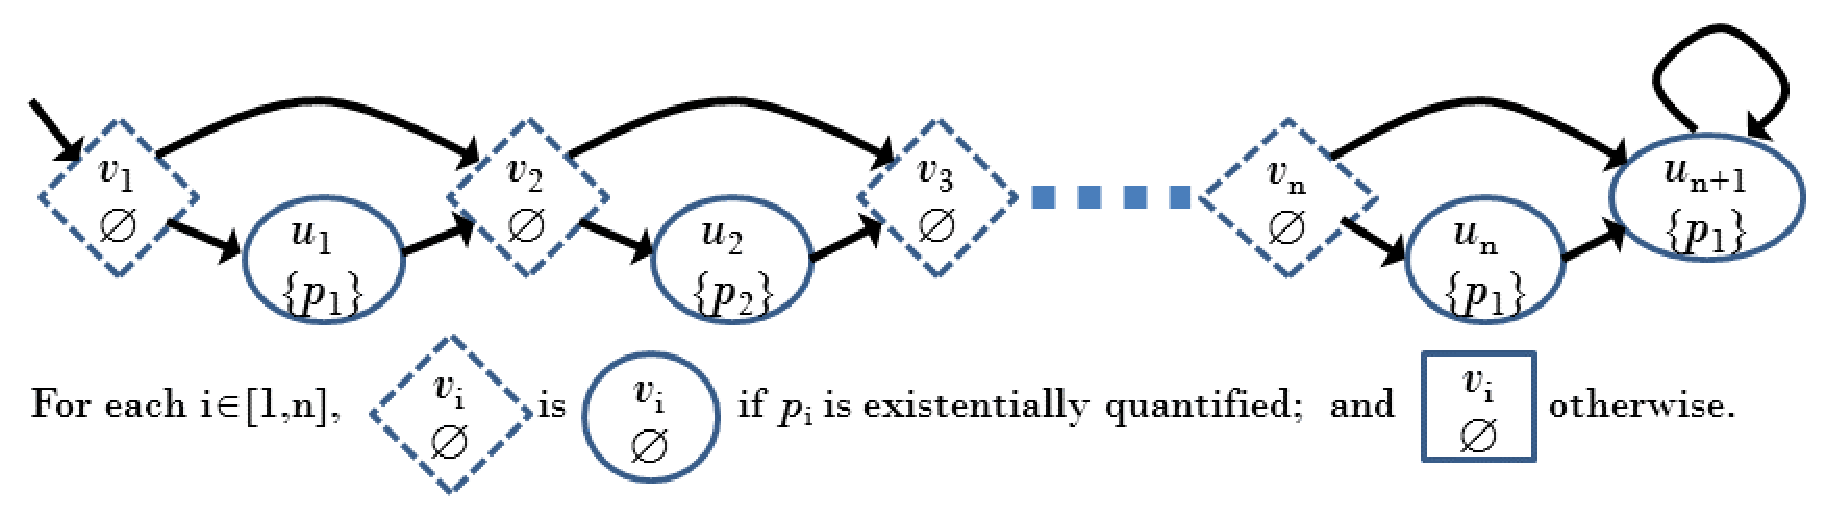
\epsfig{file=gg.altp.eps,width=150mm} 
% \input{gg.atlp.psp80.tex}
\\
$\bigcirc$ belongs to Agent 1 and $\pfrr$ belongs to Agent 2.
\end{center}
\caption{Game graph for the PSPACE-hardness proof of a Boolean formula
with $n$ propositions}
\label{fig.gg.bsil.nphard}
\end{figure}

In the graph, we use oval nodes for states owned by Agent 1 and 
square nodes for states owned by Agent 2.
In each state, we put down its name and the set of atomic
propositions that are true at the node.
For each atomic proposition $p_i\in P$,
we have a corresponding subgraph consisting of nodes
$v_i$ and $u_i$.
The subgraph of $u_i$ corresponds to $\Gamma_{p_i}$ and
and that of $v_i,u_i$ together corresponds to $\Omega_{p_i}$.  

The design of the graph allows only at most one visit
to states $v_1,\ldots,v_n$.
For all $i\in[1,n]$, state $v_i$ is owned by Agent 2 if $p_i$ is
universally quantified;
and owned by Agent 1 otherwise.
If $p_i$ is owned by Agent 1,
then Agent 1 can choose either
$(v_i,u_i)$ or $(v_i,v_{i+1})$.
If $p_i$ is owned by Agent 2,
then both choices of Agent 2 at node $v_i$ must yield
satisfaction of $\eta$.

We construct an ATL$^+$ formula $\phi_\eta$
as % follows.
% \begin{center}
$\langle 1\rangle \bigwedge_{1\leq i\leq k}
\bigvee_{1\leq j\leq h_k} \tau(l_{i,j})$ 
% \end{center}
where $\tau(p)\defn \pevt p$ and $\tau(\neg p)\defn \pfrr \neg p$. 
I.e., $\phi_\eta$ is obtained from $\eta$ by replacing the leading quantifiers in $\eta$ by $\langle 1 \rangle$.

We now show that $\calg_\eta \models \phi_\eta$ if, and only if, $\eta$ is satisfied (i.e., if $\eta$ is a tautology).
The  latter is the case if there is a winning strategy for a `satisfier' in the following game between a `satisfier' and a `refuter':
following the order of the bound variables, the `satisfier' and `refuter' choose the truth value of the existentially and universally bound variables, respectively.
When all variables are assigned truth values, the `satisfier' wins if the CNF formula is satisfied with these values. Otherwise, the refuter wins.

Taking a winning strategy of the satisfier in this game obviously provides a winning strategy for Agent 1 and, vice versa, a winning strategy of Agent 1 in the model checking game can be used as a winning strategy for the `satisfier' in the satisfaction game.
\qed

We have an example for the reduction in the proof 
of Lemma~\ref{lemma.bsil.mck.nphard}.  

{\example \label{exmp.bsil.nphard}:}
Given
$\eta\equiv \exists p\forall q\exists r
((p\vee q \vee r)\wedge(\neg p \vee \neg r))$,
according to the construction
in the proof of Lemma~\ref{lemma.bsil.mck.nphard},
we have the following ATL$^+$ formula:
$\phi_\eta\defn 
\langle1\rangle(((\pevt p)\vee (\pevt q) \vee (\pevt r))
  \wedge((\pfrr\neg p) \vee (\pfrr\neg r)))$.
\qed

Following Lemmas~\ref{lemma.bsil.mck.nphard} and
\ref{lemma.alg.pspace}, we obtain the complexity of our model-checking problems.

{\lemma\label{lemma.bsil.pspace.complete} The BSIL and ATL$^+$ model-checking
problems are PSPACE-complete.
} \qed



\section{Automata for BSIL model-checking
\label{sec.mck.gen}
}

In this section, we discuss a simple encoding of BSIL model-checking 
in {\em alternting automatas} on infinite trees 
\cite{Kirsten02,Zappe02}.  
This naturally raises the question why we should study 
a second approach to BSIL model-checking.
The answer is twofold.
First, for model-checking itself, 
it will allow us to establish that the model complexity 
of BSIL model-checking is polynomial time complete:
the problem to decide for a fixed BSIL formula $\phi$ whether 
or not a game graph $\calg$ is a model of $\phi$ is P complete.
As it is widely believed that models are usually large 
while specifications are small, a polynomial time bound in the size 
of the model might be considered more attractive than a PSPACE bound 
on the complete input.
Second, it provides us with the full access of automata 
based analysis tools, which will allow us to establish 
a doubly exponential upper bound on the decision problem of whether 
or not a BSIL formula $\phi$ is satisfiable.

We start this section by introducing alternating automata, 
and then continue to encode the model-checking algorithm 
from the previous section.
These automata constructions are then used to establish 
the inclusion of the model-checking algorithm in PTIME 
for fixed formulas, 
while hardness is shown by reducing reachability 
in AND/OR graphs \cite{Immerman81} to model-checking the BSIL formula 
$\langle 1 \rangle \pevt p$.
Beyond establishing PTIME inclusion, 
we actually show that the problem is fixed parameter tractable: 
the problem is, for a fixed formula, only quadratic in the size 
of the model.


\subsection{Alternating Automata (AA)}

{\em Alternating automata} ({\em AA}) are used 
to recognized $\omega$-regular 
tree languages over labeled trees.  
Let $\nnneg$ denote the set of non-negative integers.  
Let $\bbbbd=[1,d]$ be an interval of $\nnneg$.   
A $\bbbbd$-tree $T$ is a non-empty prefix-closed subset of $\bbbbd^*$ 
(and hence $T \subseteq \bbbbd^*$).  
In $T$, $\bbbbd$ can be interpreted as {\em directions} from 
each node in $T$.  
Such a $T$ is an ordered tree in the sense that 
the children of a node in $T$ are naturally ordered according to 
the directions in $\bbbbd$.   
For example, when $d=5$, 
the children of $1212$ can be $12122$, $12123$, and $12125$ in order. 

An $X$-labeled tree of $\Upsilon$ is a pair $\langle T,\xi\rangle$, 
where $\xi:T\rightarrow X$ is a function from $T$ to $X$.  
We use $\bbbbb^+(P)$ to denote the 
set of positive\footnote{A Boolean formula is positive if there is 
no negation in the formula.} 
Boolean combinations of elements in $P$.  
A satisfying assignment to a formula in $\bbbbb^+(P)$ is 
a subset of $P$ such that 
the formula is true if, and only if, 
all elements in the set is interpreted true.  

For the convenience of the readers, we briefly review the 
definition of AA.  

\begin{definition}  
An alternating automaton ({\em AA}) 
$A$ is a tuple $\langle X,U,u_0,\delta,\gamma\rangle$, such that
\begin{list1} 
\item $X$ is the set of labels of the analysed trees,
\item $U$ is a finite set of states,
\item $u_0\in U$ is an initial state, 
\item $\delta:(U\times X)\mapsto \bbbbb^+(\bbbbd\times U)$ 
  is a function that maps each pair of a state in $U$ 
  and an input letter in $X$ to 
  a positive Boolean combination of pairs of directions and states, and
\item $\gamma:U\mapsto \nnneg$ is a valuation function that 
  labels each state with a non-negative integer, called its {\em priority}.  
\end{list1} 
Alternating automata are interpreted over $X$-labeled trees.
A \emph{run} of $A$ 
on an $X$-labeled tree $\Upsilon=\langle T,\xi\rangle$ is a tree 
$\langle T',\xi' \rangle$ 
with $\xi':T' \mapsto (T\times U)$ with the following 
inductive restrictions. 
\begin{list1}
\item $\xi'(\varepsilon)=(\varepsilon,u_0)$.  
  $\varepsilon$ is the null sequence. 
\item For every $u\in U$ and sequence $\zeta\in T$ and $\zeta'\in T'$ 
  with $\xi'(\zeta')=(\zeta,u)$ and $\xi(\zeta)=x$, 
  there is a satisfying assignment 
  $S$ of $\delta(u,x)$ such that 
  for every $(i,u')\in S$, there exists a $k\in\nnneg$ with 
  $\zeta'k\in T'$ and $\xi'(\zeta'k)=(\zeta i, u')$.  
\end{list1}
As can be seen, the out-degree of a node in $T'$ needs at most $d\cdot|U|$ 
while that of $T$ is at most $d$.  
\qed 
\end{definition} 


Intuitively, we want to 
construct AAs with {\em states} representing path obligations.  
The transitions then define in which way these path obligations 
are sent down the tree.  
An element $(i,u')$ in the transition formula 
simply means that the path obligation from $u$ is sent to 
the child state $u'$ at direction $i$ of the input $X$-labeled tree.  

The priority of a node in a run tree is the priority of 
the state in its label.
The priority of an infinite path is the highest priority taken by infinitely many nodes on the path.
A run tree is accepting if the priority of all infinite paths are even, and a tree is accepted if it has an accepting run.
The set of trees accepted by such an automaton is called its language and an automaton is called empty if its language is empty.

An AA is called {\em nondeterministic} 
if all functions in the image of $\delta$ 
can be written as a disjunction over conjuncts 
that contain at most one pair per direction.
If they contain only one such disjunct, 
it is called {\em deterministic}.

An AA is called a \emph{safety} AA if all its states have 
the same even priority.  
For safety AA, the priority function is therefore omitted.
An AA is called \emph{weak} if for all its states $u$ 
and all input letters $x$, 
the function $\delta(u,x)$ refers only to states with priorities greater 
or equal to $\gamma(u)$.  
It is called a \emph{B\"uchi} AA if only prioritiy values $1$ and $2$ 
are used, i.e., the image of $\gamma$ 
is contained in $\{1,2\}$.  
Note that weak AA can be rewritten as language equivalent B\"uchi AA 
by changing only the priority function from $\gamma$ to $\gamma'$ 
where $\gamma'$ maps a state $u$ to $2$ if $\gamma(u)$ is even, and 
to $1$ otherwise. 




\subsection{Model Checking with AA's}

In this subsection, we relate the algorithms 
used for model-checking from Section~\ref{sec.mck.psp} 
to alternating automata.
In order to approach this translation, 
we start with the simple case where we model check a tree, 
against a BSIL formula of the form $\langle A \rangle \tau$, 
where $\tau$ does not contain an SQ.  
This is plausible since we can evaluate those SQs and replace them 
with auxiliary propositions.  
In addition, we assume that all strategy decisions are already made.  
This is also reasonable since we only allow existential SIQs and 
we forbid negations directly applied to SIQs.  
Thus we can check the model by checking the existence of S-profiles that 
fulfill the SQs and SIQs.  
For convenience, we let $\bbbbs$ be the set of strategies that 
fulfills the SQs and SIQs, if existent. 

Like in Section~\ref{sec.mck.psp}, 
we start with the case that the DNBB formula has only one disjunct.
For this case, we model check a tree that has the form 
of an unravelling of $\calg$.
To relate this to the automata we have introduced, 
we assume for the moment that the successors are ordered: 
a tree node with $k$ successors has a successor in direction $1$ through $k$.
Each node is labelled with a triple $(a,k,S,P)$, 
containing the following information:
\begin{itemize}
\item $a \in [1,m]$ shows the owner of the node,
\item $k \in \bbbbd$ shows the number of successors, and
\item $S\subseteq \bbbbs$ is the set of strategies, 
  for which we can reach the node.
  The strategies in $S$ are used just like atomic propositions.
\item $P$ is the set of atomic propositions valid in the node.
\end{itemize}
For such a tree, we check two things for the satisfaction of 
a BSIL property:
\begin{list1}
\item[(A1):] The labelling of states as reachable is consistent; 
  that is, there are strategies in $S$ such that, 
  for each strategy, exactly the nodes labelled by it are reachable.
\item[(A2):] For the respective set of paths described by this labelling, 
  the single disjunct of the DNBB is satisfied.
\end{list1}  
Note that, by these, we do not check that the form of 
the tree complies with an unravelling of $\calg$.
%
However, the following observation obviously holds.

{\lemma \label{lemma.A1.A2} 
$\calg$ is a model of $\phi$ if, and only if, 
we can extend the unravelling of $\calg$ such that (A1) and (A2) 
are satisfied.
} 
\qed 

To test this, we will first show how to construct two AAs that 
check (A1) and (A2) individually, and 
then construct a nondeterministic B\"uchi AA that checks (A1) and (A2) 
together.
Using a nondeterministic AA is attractive because it allows 
for projecting away the strategies and interpreting $\calg$ directly 
with the resulting AA.

{\lemma \label{lemma.A1} 
We can construct a nondeterministic safety AA 
$\cala_s=\langle X,U_s,u_0^s,\delta^s \rangle$ 
with $2^{|\bbbbs|}$ states that recognises 
the trees that satisfy (A1).
}
\\\pf 
We can simply use 
$X = [1,m] \times \bbbbd \times 2^\bbbbs \times 2^P$,
$U_s = 2^\bbbbs$, and 
$u_0^s = \bbbbs$.   
For all $k \leq d$, we have a transition function 
$\delta_k^s$ for the $k$ successor case (of the input labeled tree node) 
with the following restrictions. 
\begin{list1}
\item For an Agent $a$ owning a state and a set of strategies 
  $S \subseteq \bbbbs$, we let
  $S_a \subseteq S$ be the strategy names of strategies 
  for Agent $a$.  
  We let $\Pi^k_a=\{S_a^1,S_a^2,S_a^3,\ldots, S_a^k\}$ be a disjoint cover of $S_a$
  and $S^\neg_a = S - S_a$ be the set of strategies not owned by $a$.  
\item We let $\delta_k^s(a,S) = \bigvee_{S_a^1,\ldots,S_a^k\in \Pi_a^k}
  \bigwedge_{i\in [1,k]}(i,S_a^i\cup S^\neg_a)$.  
  Then we let $\delta_s \big(S,(a,k,S,P)\big) = \delta_k^s(a,S)$ 
  and \linebreak 
  $\delta_s \big(S,(a,k,S',P)\big)=\false$ if $S\neq S'$.
\end{list1}
First, the automaton is nondeterministic, and it is easy to see that a run tree must have the same form and the states in its nodes must comply with the strategies in the label of the input tree.

With this observation, the correctness of the construction can be shown by a simple inductive argument.
For the induction basis, the initial node is reachable under all strategies, and the run tree is labeled with all strategies.
For the induction step, it is easy to show by induction that a node of a (minimal) run tree (and, similarly, the input tree) must have the following property.
\begin{list1}
 \item If a state is not labelled with a strategy $s_i$, then no successor is labeled with $s_i$.
 \item If a state is labelled with a strategy $s_i$ owned by a different agent than the node, then all successor states must be labeled with $s_i$.
 \item If a state is labelled with a strategy $s_i$ owned by the same agent as the node, then all exactly one successor state is labeled with $s_i$.
\end{list1}
Also, any combination of the labels according to the last rule is possible.
This exactly characterize the labelling of reachability for the different strategies.
\qed 



Now we want to construct a weak deterministic AA for property (A2).  
Let $\bbbbc$ denote the set of BP-obligations from property (A2).

{\lemma \label{lemma.A2} 
We can construct a weak deterministic automaton 
$\cala_\wedge=\langle X,U_\wedge,u_0^\wedge,\delta_\wedge, \gamma_\wedge 
\rangle$ with $2^{|\bbbbc|}$ states that recognises the run trees 
that satisfy (A2).
}
\\\pf 
We can simply use
$X = [1,m] \times \bbbbd \times 2^\bbbbs \times 2^P$,
$U_\wedge = 2^\bbbbc$, and 
$u_0^\wedge = \bbbbc$.  
For the transition formulas, 
we have the following restrictions. 
\begin{list1} 
\item $\delta_\wedge \big(C,(a,k,S,P)\big) =\false$ 
  if there exists a $\Lambda\theta\in C$ with $\Lambda\not\subseteq S$.  
  That is, we require that all transitions can only use strategies 
  that have been passed down from the ancestors.  
\item $\delta_\wedge \big(C,(a,k,S,P)\big) =\false$ 
  if there exists a $\Lambda\theta\in C$ with $\tteval(P,\theta)=\false$.  
  Please recall that $\tteval(P,\theta)$ 
  converts a $\theta$ that is locally violated by $P$ to $\false$.  
\item Otherwise, $\delta_\wedge \big(C,(a,k,S,P)\big)
  =\bigwedge_{i\in[1,k]} (i,C')$ with 
  $C' = \{\Lambda\ttnxt(\tteval(P,\theta))\mid \Lambda\theta \in C\}$.  
\end{list1} 
Note that $\cala_\wedge$ is made deterministic by encoding 
the choices of strategy passing-down in the input symbol $(a,k,S,P)$.  
Then we define $\gamma_\wedge$ such that $\gamma_\wedge(C)$ 
is odd iff $C$ contains an until formula $\phi_1 \until \phi_2$.
The correctness of the construction is straightforward.  
\qed 


Intersection of $\cala_s$ and $\cala_\wedge$ can, 
as usual, be done on the state level.

{\corollary \label{coro.aa.Ap}
We can construct a nondeterministic weak AA 
$\cala'=\langle [1,m] \times \bbbbd \times 2^\bbbbs \times 2^P,U,u_0,\delta', \gamma \rangle$ 
with $2^{|\bbbbs|+|\bbbbc|}$ states 
that recognises trees that satisfy (A1) and (A2).
}
\\\pf 
The new state set $U$ are simply $U_s \times U_\wedge$ and 
the initial state is $(u_0^s,u_0^\wedge)$.   
The transition function returns false 
if either $\delta_s$ or $\delta_\wedge$ return false, 
and are applied independently for the two projections otherwise.  
Finally, $\gamma(u_s,u_\wedge) = \gamma_\wedge(u_\wedge)$.
\qed 

{\corollary\label{coro.aa.A}
We can construct a nondeterministic weak automaton 
$\cala=\langle [1,m] \times \bbbbd \times 2^\bbbbs \times 2^P,
U,u_0,\delta, \gamma \rangle$ 
with $2^{|\bbbbs|+|\bbbbc|}$ states that recognises 
the trees with labelling functions that are projections from 
the trees that satisfy (A1) and (A2).
}
\\\pf 
As usual, this is achieved by choosing 
$\delta\big(u,(a,k,P)\big) = 
\bigvee_{S \subseteq \bbbbs}\delta'\big(u,(a,k,S,P)\big)$.
\qed 

The above lemmas and corrolaries  
make it easy to proof our major claim in the section.  

{\theorem\label{thm.aa.main}
Model-checking BSIL formulas can be done in time exponential in the BSIL formula and bilinear in the number of states and transitions of the model.
}
\\\pf 
Corollary~\ref{coro.aa.A} 
establishes this for PSIL formulas of the form 
$\phi=\langle A \rangle \tau$, where $\tau$ does not contain any SQ.
We can extend this to general BSIL state formulas with the following 
steps. 
\begin{stmt1} 
\item First, this extends to the case of several disjuncts simply 
  by checking the claim for each disjunct individually.
\item Second, we can model check this for any state (treating it as the initial state) and subsequently store the result by introducing a fresh atomic proposition $p_\phi$, and replace the sub-formula $\phi$ in the specification by $p_\phi$.
\item Repeating the above two steps until we have reduced 
  the model-checking problem to model-checking a Boolean formula.
\end{stmt1} 
This procedure requires the model-checking procedure 
to be repeated for every SQ as many times as $\calg$ has states.
(In principle, it would suffice for the topmost SQ to model check it 
for only the initial state.)

The model-checking algorithm for each state and SQ requires 
to run up to the number of disjuncts many times the respective 
consgtruction algorithm of $\cala$.
We can assume without loss of generality that the turn-based game structure is properly labeled, as it contains a label for the ownership as well as a label for the atomic propositions, so we only have to add a label for the number of successors and number the directions.

The na\"ive approach of playing the acceptance game by 
offering an acceptance player the choice of a disjunct 
and a rejection player the choice of a direction is obviously too expensive. 
But note that we can split the decision as follows. 
\begin{list1}
\item Let the acceptance player choose the set $S$ 
  from $\delta\big(u,(a,k,P)\big) = 
  \bigvee_{S \subseteq \bbbbs}\delta'\big(u,(a,k,S,P)\big)$,
\item Let the acceptance and rejection player choose 
  $\delta_s^k(a,S)$ successively by, starting with 
  $I_0=\bbbbd$ and $S_0 = S_a$.  
  Then we use binary search style to iteratively 
  narrow down $I_0,I_1,\ldots$ by repeating the following steps for  
  $i=0,1,2,\ldots$:  
  \begin{stmt1}
  \item Cut $I_i = [l,u]$ with $m=\big\lfloor\frac{l+u}{2}\big\rfloor$ 
    into $I_i^l = [l,m]$ and $I_i^u = [m+1,u]$.   
  \item Let the acceptance player choose disjoint sets $L_i$ and $U_i$ 
    whose union is $S_i$.    
  \item Let the rejection player choose to continue 
    with either $I_{i+1}= I_i^l$ and $S_{i+1} = L_i$, 
    or with $I_{i+1}= I_i^u$ and $S_{i+1} = U_i$.  
  \end{stmt1}
  The repetition goes on until 
  $I_i =\{j\}$ is singleton and then execute 
  $\big(j,S_i \cup (S - S_a)\big)$.
\end{list1}
That is, by approaching the chosen transition in a logarithmic search we can avoid the overhead. Solving this game is linear in its state space, and this is linear in the number of transition of $\calg$.
\qed 





For PTIME hardness, we reduce the reachability checking 
in an AND/OR graphs \cite{Immerman81} to model-checking for the simple BSIL formula $\langle 1 \rangle \pevt p$.
For the reduction, it suffices to turn AND nodes to nodes owned by Agent $1$ and OR nodes to nodes owned by Agent $2$.

{\theorem\label{thm.aa.lb} 
Model-checking BSIL formulas is PTIME complete in the size of the model.
}
\qed 




\section{BSIL Satisfiability\label{sec.sat}} 


In this section, we show that the satisfiability problem of BSIL is 2EXPTIME complete.
The upper bound can be inferred by the simulation theorem \cite{}, while hardness is a consequence of the inclusion of CTL${}^+$.

In the first step, 
we provide an AA for checking the consistency of a labelling 
as it is constructed in the model-checking approach in the previous section.
This labelling contains explicit information about whether 
or not a BSIL SQ formula is satisfiable.
In the following we assume without loss of generality 
that every state in the turn based game is reachable from 
the initial state without mentioning this explicitly.
(Note that unreachable states have no impact on the correctness 
and can simply be removed.)



{\lemma\label{lemma.sat.B}
We can build an AA $\calb$ 
which is exponential in the size of a BSIL formula $\chi$ 
and accepts a fully labelled turn-based game 
iff the labelling is consistent and the turn-based game structure 
is a model of $\chi$.
}
\\\pf 
For each SQ subformula $\phi$ of $\chi$, 
we can build a weak nondeterministic AA 
$\cala_\phi$ that consists of the nondeterministic AA 
$\cala_\eta$ for each disjunct $\eta$ in the DNBB formula of $\phi$ 
(where we assume, without loss of generality, 
that their states are disjoint and 
$\cala_\eta$ has initial state $u_\eta$) 
plus a fresh initial state $u_0$ with priority $0$.
The transition function for $u_0$ is simply
$\delta(u_0,x) = \bigvee_{\eta} \delta(u_\eta,x)$, 
that is, in the first step one arbitrary individual automata 
is entered and never left again.

Likewise, we can build a weak AA $\cald_\phi$ 
that accepts the complement language of $\cala_\phi$ 
by dualising it.  
Let $K$ denote the set of subformulas of $\chi$ that start with an SQ.
Assume, without loss of generality, 
that the states of the individual $\cala_\phi$ and $\cald_\phi$ 
are disjoint and 
that the initial states of $\cala_\phi$ and $\cald_\phi$ are $u_\phi$ 
and $\overline{u}_\phi$, respectively.
Then we can build $\calb$ by adding two fresh states, a state $u$ 
and the initial state $u_0$ (both with priority 0) and define 
the transition formula as follows. 
\begin{list1}
\item $\delta\big(u_0,(a,k,P)\big) =$ \emph{false} if $P\not\models \chi$ 
  and  
\item $\delta\big(u_0,(a,k,P)\big) = \delta\big(u,(a,k,P)\big)$ 
  if $P\models \chi$,
\item $\delta\big(u,(a,k,P)\big) = \bigwedge\limits_{i\in[1,k]}(i,u) 
  \wedge \bigwedge_{\phi\in K,p_\phi\in P} \delta\big(u_\eta,(a,k,P)\big) 
  \wedge \bigwedge_{\phi\in K,p_\phi\notin P} 
    \delta\big(\overline{u}_\eta,(a,k,P)\big)$.
\end{list1}
For the states of the individual $\cala_\phi$ and $\cald_\phi$, their transition and priority function is used.
\qed 


{\theorem\label{thm.sat}
The satisfiability of a BSIL formula $\phi$ can be checked in time doubly exponential in the size of $\varphi$.
If $\varphi$ is satisfiable, then a model can be constructed in time doubly exponential in $\varphi$.
}
\\\pf
The main difference to the model-checking case is that we cannot infer a sufficient branching degree from the model.
We therefore approach in two steps: we assume that we know a sufficient branching degree, and discuss a synthesis algorithm for it.

The first observation is that, for states in a $\cald_\phi$, 
we can use any subtree as this automaton shows that something holds 
for all strategies.   
The reduction to a subtree makes the property easier to satisfy.
The second observation is that a winning strategy 
for the acceptance player 
can be assumed to be memoryless.
Thus, for each state of an AA $\cala_\phi$ and each state 
of a tree accepted, strategies from the respective 
$S_a$ (from the proof for Lemma~\ref{lemma.A1}) 
are sent to at most $|S_a| \leq |\bbbbs|$ directions.
But successors of nodes to whom from no state a non-empty subset 
of $S_a$ is sent can be pruned, provided at least one successor remains.
This gives a bound on the number of directions needed, which is bilinear in the number of states all $\cala_\phi$ put together and the maximal number of strategies.
(The latter can be estimated by the number of SIQs bound by any SQ plus one times the number of agents.)  
Thus, the number of directions can be restricted 
to a number exponential in $\chi$.

Having established this bound of directions, 
we can build a language equivalent nondeterministic B\"uchi AA  
in time exponential in $\calb$ 
(for the given $k$-bounded branching degree), 
whose emptiness can be checked in polynomial time.
\qed




\subsection*{remark}
Strictly speaking, a specification alone does not reveal the number of agents. There are two interpretations possible: either one requires the agents to be explicitly named, or one leaves the set of agents open. In the latter case, however, all agents that are not named explicitly co-operate, and their strategy is never bound in any conjunct of a DNBB. Hence, they can be collapsed to a single agent without changing the semantics.


To obtain hardness we use draw from the 2EXPTIME-completeness of CTL$^+$.
It is easy to see that CTL${}^+$ is the sub-logic of BSIL, where $\langle A \rangle$ is restricted to $\langle \emptyset \rangle$ and $\langle+A \rangle$ operators are restricted to $\langle+\emptyset \rangle$ operators and always bind a temporal operator.
Together with the previous theorem, the 2EXPTIME hardness of CTL$^+$ \cite{} provides us with:

\begin{corollary}
Checking the realisability of a BSIL formula $\varphi$ 2EXPTIME-complete in the size of $\varphi$.
\end{corollary}



\section{Experiment \label{sec.expe}}

\subsection{Implementation} 

We implemented a semi-symbolic model checker of BSIL with {\bf REDLIB} 
\cite{Wang03,Wang08a,Wang08b,Wang13,Wang14}
which is a free library for symbolic model-checking based on decision diagrams. 
{\bf REDLIB} supports symbolic pre-condition and post-condition calculation 
of discrete transitions.  
Our model-checker starts from a symbolic representataion of the initial 
condition. 
Then it repeatedly applies the post-condition procedure of {\bf REDLIB}
to explore the symbolic state representations in the computation tree.  
Our model-checker use the result in section~\ref{sec.mck.psp} to bound 
the exploration depth of tree.   

\subsection{Benchmarks and their experiment report} 

Then we experimented with two parameterized benchmarks.  
The first is the prisoners' dilemma described in Example~\ref{exmp.pd} 
with the number of prisoners as a parameter.  
Then we applied the model checker to check whether the model  
satisfies formula (A) and (B) in the introduction.
The time and memory usage of the model checker is reported in 
Table~\ref{tab.exp.pd}.
\begin{table*}[!th]
\caption{Experiment data for the prisoners' dilemma model}
\label{tab.exp.pd}
\begin{center}
\begin{tabular}{c||c|c||c|c} \hline
\multirow{2}{*}{\#prisoners}  &\multicolumn{2}{c||}{Formula (A)} & \multicolumn{2}{c}{Formula (B)}\\ \cline{2-5}
& Time & Mem  & Time & Mem\\ \hline
2 &0.50s &72M   &0.51s &71M \\
3 &0.92s &75M   &0.88s &75M \\
4 &1.23s &83M   &1.14s &80M \\
5 &3.19s &146M  &2.90s &140M \\
6 &6.71s &388M  &6.52s &361M \\
7 &25.10s&1043M &23.11s&979M \\ \hline
\end{tabular}
\hspace*{10mm}
\parbox{50mm}{
s: seconds (computation time); \\
M: megabytes (memory usage); \\[2mm]
The experiment is conducted on a PC with Intel i7-2600k 3.4GHZ CPU 
and 8G RAM running Ubuntu 12.04. 
}
\end{center}
\end{table*}

The second benchmark is for campaign strategies 
of 2 political parties, Party $1$ and Party $2$, for seats in 
the congress.  
There are several parameters in our model, 
the number of seats in the congress, 
the amount of budget of each party in a round, 
and the number of candidates of each party in a round. 
The game is played by the chiefs of the parties, 
Chief $1$ (a gentleman) and Chief $2$ (a lady), 
who decide the amount of support that 
a candidate receive in a round.   
Candidates with more budget in a round will be elected in the round. 
If two or more candidates get the same amount of support, 
the winner will be decided randomly.  
% \begin{figure}[htb]
% \caption{Campaign Model}
% \label{exp.campaign}
% \centering
% \includegraphics[width=0.8\textwidth]{vote_example}
% \end{figure}

In our model, in each round, chief 1 first decides his budget allotment, 
then chief 2 decides her budget allotment, and 
then the election result is determined.  
For example, with 3 dollars in his budget for two candidates, 
the strategy of a Chief can be written as 
$(x,y)\in\{(3,0), (2,1),(1,2),(0,3)\}$ where $x$ and $y$ 
respectively denote the support (in dollars) 
alloted to the first and the second candidates in his party. 
If Chief $1$ uses strategy $(2,1)$ and 
Chief $2$ uses strategy $(0,2)$ (Assume she has less budget.), 
the result of the round is 
that the two parties both win one seat in the round. 
On the other hand, if Chief $2$ chooses strategy $(1,1)$ instead, 
then there is no strategy for Chief $1$ to win more seats for his party. 



We use the following propositions and predicates to write 
specifications.  
For each $i\in[1,2]$ and $j\in[1,c]$ where $c$ is the number of 
candidates, 
$\textsl{elected}_{i,j}$ means the $j$'th candidate of party $i$ is 
elected now. 
Then we can use propositions $\textsl{elected}_{i,j}$ to construct 
a predicate $\textsl{win}_i$ that means party $i$ wins more seats than party $2-i$ in the round. 
Assume that the first candidate in each party is the chief. 
Then the following BSIL formula specifies that 
Chief $1$ has a strategy to make sure candidate 1 to be elected  
and in the same time allow the opponent party to win more seats in every round.
\begin{center} 
\hfill 
$\langle 1\rangle((\langle +\rangle\pevt \textsl{elected}_{1,1})
\wedge(\langle+2\rangle\pfrr \textsl{win}_2))$
\hfill (C) 
\end{center} 
Similarly, the following formula specifies that 
the chief of party 1 has a strategy to assure that his party 
can win more seats than his opponent party while allowing party two to assure 
the winning of a candidate.  
\begin{center} 
\hfill $\langle 1\rangle((\langle +\rangle \pevt \textsl{win}_1)
\wedge(\langle +2\rangle\pevt \textsl{elected}_{2,1}))$
\hfill (D)
\end{center} 
With different values of budget and candidate count, we may use our model-checker 
to analyze the strategy for achieving various goals.  
The time and memory usage data for checking formula (C) and (D) 
is in Table~\ref{tab.exp.vote}.
\begin{table*}[!th]
\caption{Experiment Data Election}
\label{tab.exp.vote}
\begin{center}
\begin{tabular}{c|c|c|c|c||c|c|c||c|c|c} \hline
\multicolumn{5}{c||}{Parameters}
&\multicolumn{3}{c||}{Formula (C)} 
& \multicolumn{3}{c}{Formula (D)}\\ \hline
$c_1$ & $b_1$ & $c_2$ & $b_2$ & $s$ & Result & Time & Mem & Result & Time & Mem\\ \hline
2&2 &2 &4 &1 &UNSAT &0.52s &61M  &UNSAT &0.53s &61M \\
2&4 &2 &4 &2 &UNSAT &1.20s &75M  &UNSAT &1.15s &75M \\
2&4 &2 &4 &3 &SAT   &0.73s &75M  &UNSAT &1.14s &75M \\
3&6 &3 &6 &3 &SAT   &1.51s &211M &UNSAT &0.93s &211M \\
3&9 &3 &6 &3 &UNSAT &9.14s &837M &SAT   &5.22s &681M \\
3&6 &3 &9 &3 &SAT   &8.74s &502M &UNSAT &8.49s &502M \\
3&9 &3 &9 &4 &SAT   &158s  &6631M&UNSAT &93.17s&5082M \\ \hline
\end{tabular}
\hspace*{2mm}
\parbox{75mm}{
$c_1$: \# candidates of party 1\\
$b_1$: total budget in a round of party 1\\
$c_1$: \# candidates of party 2\\
$b_1$: total budget in a round of party 2\\
$s$: \# of seats in the congress\\[2mm] 
s: seconds (computation time)\\
M: megabytes (memory usage) \\[2mm]
The experiment is conducted on a PC with Intel i7-2600k 3.4GHZ CPU 
and 8G RAM running Ubuntu 12.04. 
}
\end{center}
\end{table*}

The experiment data shows that our tool can be used in analyzing strategies 
for winning games.  
It would be interesting to see how general and specific 
performance improvement techniques could be designed in the future fro 
practical industry projects.  



\section{Conclusion \label{sec.conc}}

BSIL can be useful in describing close collaboration among strategies of 
agents in a multi-agent system. 
Although it can express properties that
ATL$^*$, GL, and AMC cannot, its model-checking problem incurs a
much lower complexity.  
Future work in this direction may include
further extension to BSIL and 
better efficient model-checking algorithms.  

\section*{Acknowledgment}
The authors would like to thank Moshe Vardi and the anonymous reviewers of CONCUR 2011 for their valuable comments and suggestions. 



\bibliographystyle{abbrv}
\bibliography{../../../valcite}





\end{document}
